% !TeX root = thesis.tex
\chapter{Results}
This chapter presents the main results for CAGNN and the baseline models under the warm, cold drug target, and cold cell splits. The results are organized into error, correlation, top gene precision, direction of change, ablation, uncertainty, data efficiency, and case studies.

\section{Evaluation framework}
\noindent All experiments in this chapter use the L1000 landmark setting with 978 genes. For every sample, the prediction target is the response vector $y = x_{\mathrm{trt}} - x_{\mathrm{ctl}}$. All models use the matched control profile and the drug input. CAGNN also uses cell context information.

\noindent The evaluation compares three models, namely the DeepCOP style baseline with dense layers, GSNN \cite{evans2024gsnn} as the graph based baseline, and Counterfactual Attention GNN (CAGNN). The split settings, pairing rules, and metric definitions are introduced in the Evaluation Metrics section of the methodology chapter. The same evaluation framework is used here to compare the models.

\noindent Most tables and figures in this chapter show the main comparison between CAGNN and the baseline models. Later sections then switch to additional analyses. The ablation section compares cell identity and control derived cell context within CAGNN. The uncertainty section studies the uncertainty output of the same CAGNN model. The data efficiency section studies warm split training budgets only. The case study section uses selected CAGNN examples to help explain the model behavior.

\begin{table}[htbp]
\centering
\caption[Evaluation Protocol Summary]{Summary of the evaluation protocol used in the thesis.}
\label{tab:result_protocol}
\begin{tabular}{p{3.0cm}p{9.2cm}}
\hline
Component & Setting \\
\hline
Dataset & LINCS L1000 landmark genes, 978 genes \\
Prediction target & Differential response $y = x_{\mathrm{trt}} - x_{\mathrm{ctl}}$ \\
Models & DeepCOP baseline, GSNN, CAGNN \\
Splits & Warm, cold drug target, cold cell \\
Primary metrics & Test MSE, test PCC averaged across samples, sign accuracy, Pos P@20, and Neg P@20 \\
Top gene analysis & Pos P@20 and Neg P@20 \\
Additional analyses & Ablation, uncertainty, data efficiency, and case studies \\
Attention analysis & Case study on specific drug\\
\hline
\end{tabular}
\end{table}

\begin{figure}[htbp]
\centering
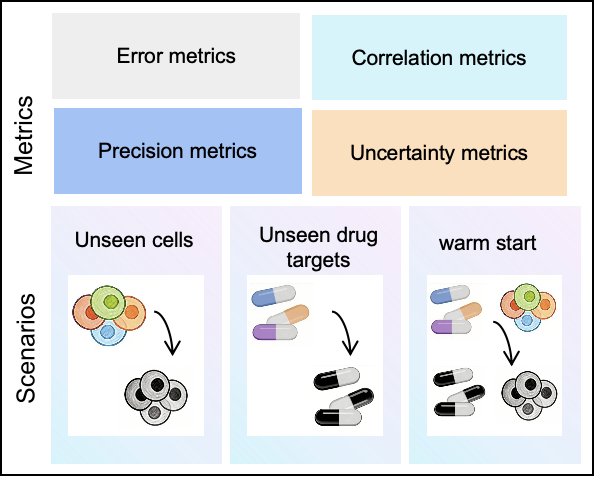
\includegraphics[width=0.615\linewidth]{figures/evaluation_framework.png}
\caption[Evaluation Configuration]{Simple view of the evaluation configuration used in this chapter.}
\label{fig:evaluation_framework}
\end{figure}

\noindent Figure~\ref{fig:evaluation_framework} shows the three split settings, the main metric groups, and the overall comparison logic. The later sections follow this same layout.


\section{Error metric results}
\noindent Error metrics measure how close the predicted values are to the observed values. The main error metric here is mean squared error (MSE), where a lower score means a better prediction. Table~\ref{tab:mse_results} and Figure~\ref{fig:benchmark_mse_results} show the same ranking in table and plot form. CAGNN gives the lowest MSE in warm and cold drug target, while DeepCOP is slightly best in cold cell. The clearest separation appears in cold drug target, whereas cold cell shows a smaller gap and a different ranking.

\begin{table}[htbp]
\centering
\caption[Test MSE Across Splits]{Test MSE under the three evaluation splits. The best value in each split is shown in bold.}
\label{tab:mse_results}
\begin{tabular}{lccc}
\hline
Split & DeepCOP & GSNN & CAGNN \\
\hline
Warm & 0.8915 & 0.9609 & \textbf{0.8182} \\
Cold drug target & 1.5109 & 1.4297 & \textbf{1.3228} \\
Cold cell & \textbf{0.8133} & 0.8466 & 0.8384 \\
\hline
\end{tabular}
\end{table}

\begin{figure}[htbp]
\centering
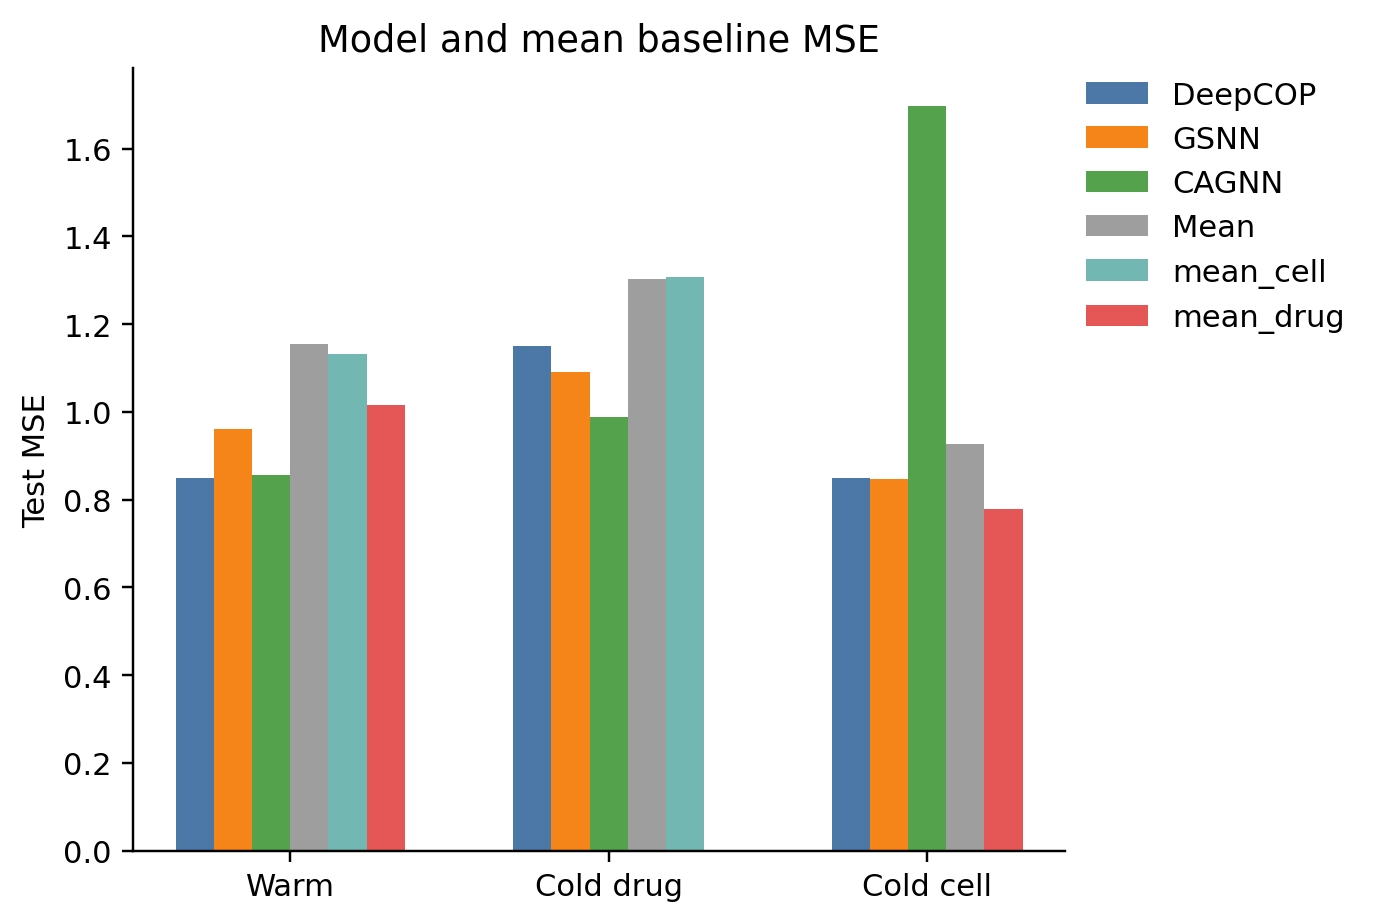
\includegraphics[width=0.86\linewidth]{figures/benchmark_mse_with_mean_baselines.png}
\caption[MSE with Mean Baselines]{Test MSE in warm, cold drug target, and cold cell for the learned models and the simple mean baselines. mean\_drug is not shown in cold drug target and mean\_cell is not shown in cold cell because these baselines cannot be used there.}
\label{fig:benchmark_mse_results}
\end{figure}

\noindent Scatter plots of $y_{\mathrm{true}}$ and $y_{\mathrm{pred}}$ show this ranking more clearly. Points close to the diagonal indicate smaller errors, while a wider cloud indicates larger deviations. In Figure~\ref{fig:gene_expr_true_pred}, the CAGNN panels are tighter around the diagonal in warm and cold drug target than the baseline panels. In cold cell, the point clouds become wider for all three models and the differences become smaller. This matches Table~\ref{tab:mse_results}.

\begin{figure}[htbp]
\centering
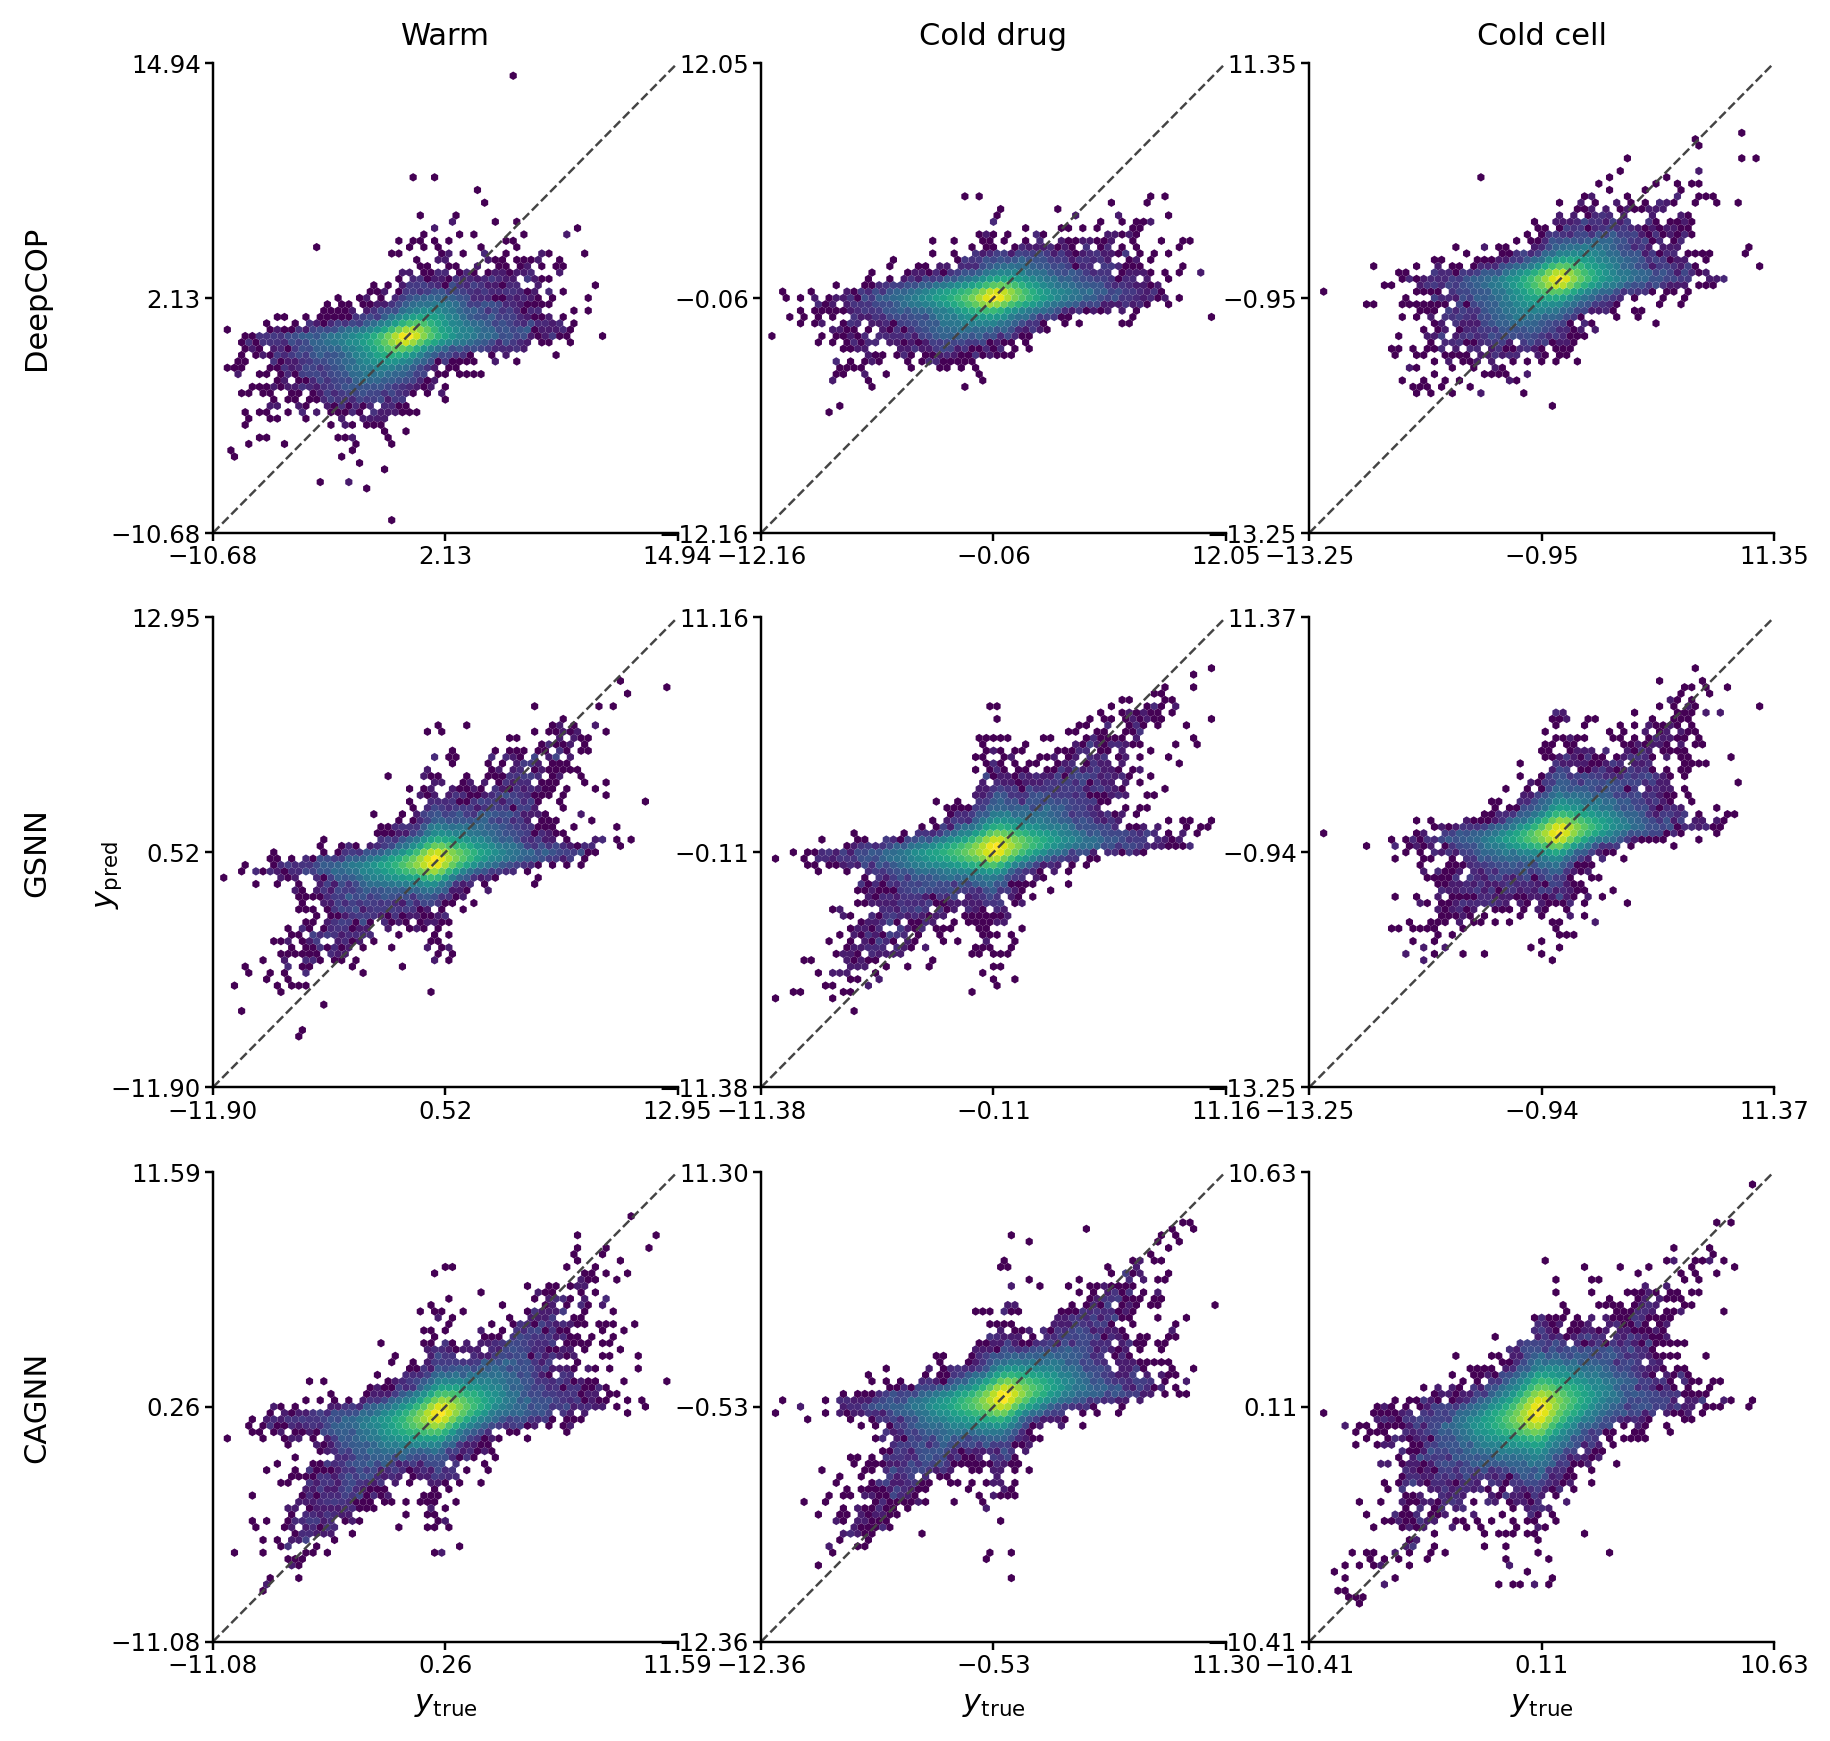
\includegraphics[width=0.882\linewidth]{figures/gene_expr_true_pred_all_models_by_split.png}
\caption[Gene Scatter Plots]{Scatter plots of predicted and true values for individual genes for DeepCOP, GSNN, and CAGNN in the three splits.}
\label{fig:gene_expr_true_pred}
\end{figure}

\FloatBarrier
\section{Precision metric results}
This part examines whether the models recover the strongest changes across genes. The evaluation uses top gene precision, which emphasizes the genes with the largest positive and negative responses.

\noindent For each sample, the genes are ranked in both the true response ($y_{\mathrm{true}}$) and the predicted response ($y_{\mathrm{pred}}$). Positive precision at 20, written as Pos P@20, measures how many of the 20 most up regulated genes in $y_{\mathrm{pred}}$ also appear among the top 100 most up regulated genes in $y_{\mathrm{true}}$. Negative precision at 20, written as Neg P@20, is defined in the same way for the 20 most down regulated genes. The final score is the mean across all test samples. These metrics give another view of prediction quality that is closer to how perturbation results are often used in practice.

\noindent Table~\ref{tab:top_gene_analysis} and Figure~\ref{fig:top_gene_placeholder} show the same result in table and plot form. CAGNN has the highest Pos P@20 and Neg P@20 in every split. The advantage is clear in warm and cold drug target, and it remains visible in cold cell.

\begin{table}[!htbp]
\centering
\caption[Top Gene Precision Results]{Top gene precision results computed from the exported prediction files. The best value in each split is shown in bold.}
\label{tab:top_gene_analysis}
\begin{tabular}{lccc}
\hline
Split and metric & DeepCOP & GSNN & CAGNN \\
\hline
Warm Pos P@20 & 0.5406 & 0.5179 & \textbf{0.6180} \\
Warm Neg P@20 & 0.5402 & 0.4827 & \textbf{0.6280} \\
Cold drug target Pos P@20 & 0.3892 & 0.5062 & \textbf{0.6035} \\
Cold drug target Neg P@20 & 0.4003 & 0.4855 & \textbf{0.5952} \\
Cold cell Pos P@20 & 0.4062 & 0.4779 & \textbf{0.5344} \\
Cold cell Neg P@20 & 0.4129 & 0.4388 & \textbf{0.4993} \\
\hline
\end{tabular}
\end{table}

\begin{figure}[htbp]
\centering
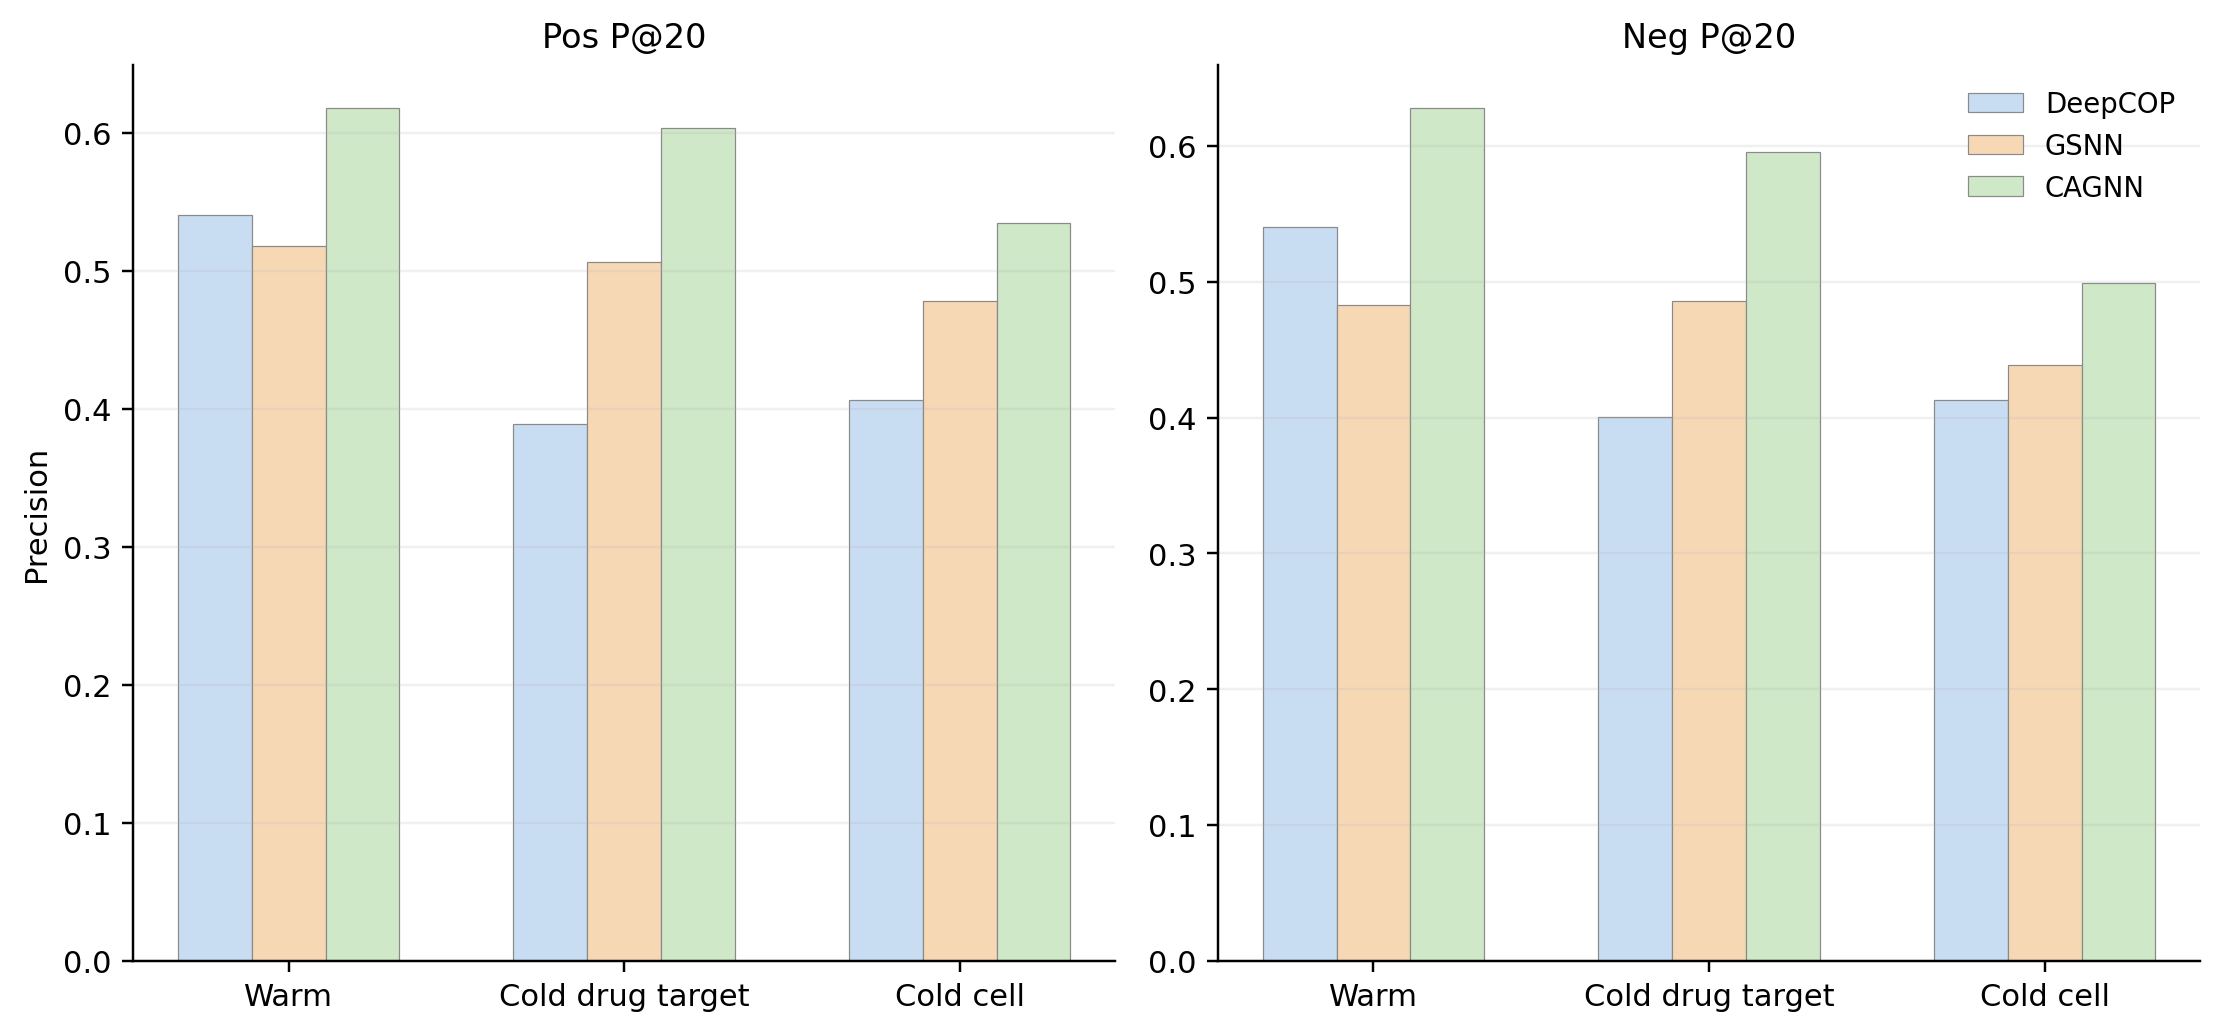
\includegraphics[width=0.86\linewidth]{figures/top_gene_precision_results.png}
\caption[Top Gene Precision Plots]{The left panel shows Pos P@20 and the right panel shows Neg P@20 for DeepCOP, GSNN, and CAGNN in the three splits.}
\label{fig:top_gene_placeholder}
\end{figure}
\FloatBarrier
\section{Correlation metric results}
The Pearson correlation coefficient (PCC) measures whether the predicted response follows the same overall pattern across genes as the true response. A higher score means better agreement in shape for each sample.

\noindent Table~\ref{tab:pcc_results} and Figure~\ref{fig:benchmark_pcc_results} show the same PCC results in table and plot form. CAGNN is highest in all three splits. The strongest baseline changes by split. DeepCOP is slightly stronger than GSNN in warm, while GSNN is clearly stronger in cold drug target and cold cell. Another clear result is that PCC decreases for all methods from warm to cold cell. In Figure~\ref{fig:benchmark_pcc_results}, the CAGNN bar is highest in each split and the cold cell bars are lower overall.

\begin{table}[htbp]
\centering
\caption[Test PCC Across Splits]{Test PCC under the three evaluation splits. The best value in each split is shown in bold.}
\label{tab:pcc_results}
\begin{tabular}{lccc}
\hline
Split & DeepCOP & GSNN & CAGNN \\
\hline
Warm & 0.4671 & 0.4609 & \textbf{0.5605} \\
Cold drug target & 0.2339 & 0.4458 & \textbf{0.5071} \\
Cold cell & 0.3457 & 0.4237 & \textbf{0.4783} \\
\hline
\end{tabular}
\end{table}

\begin{figure}[htbp]
\centering
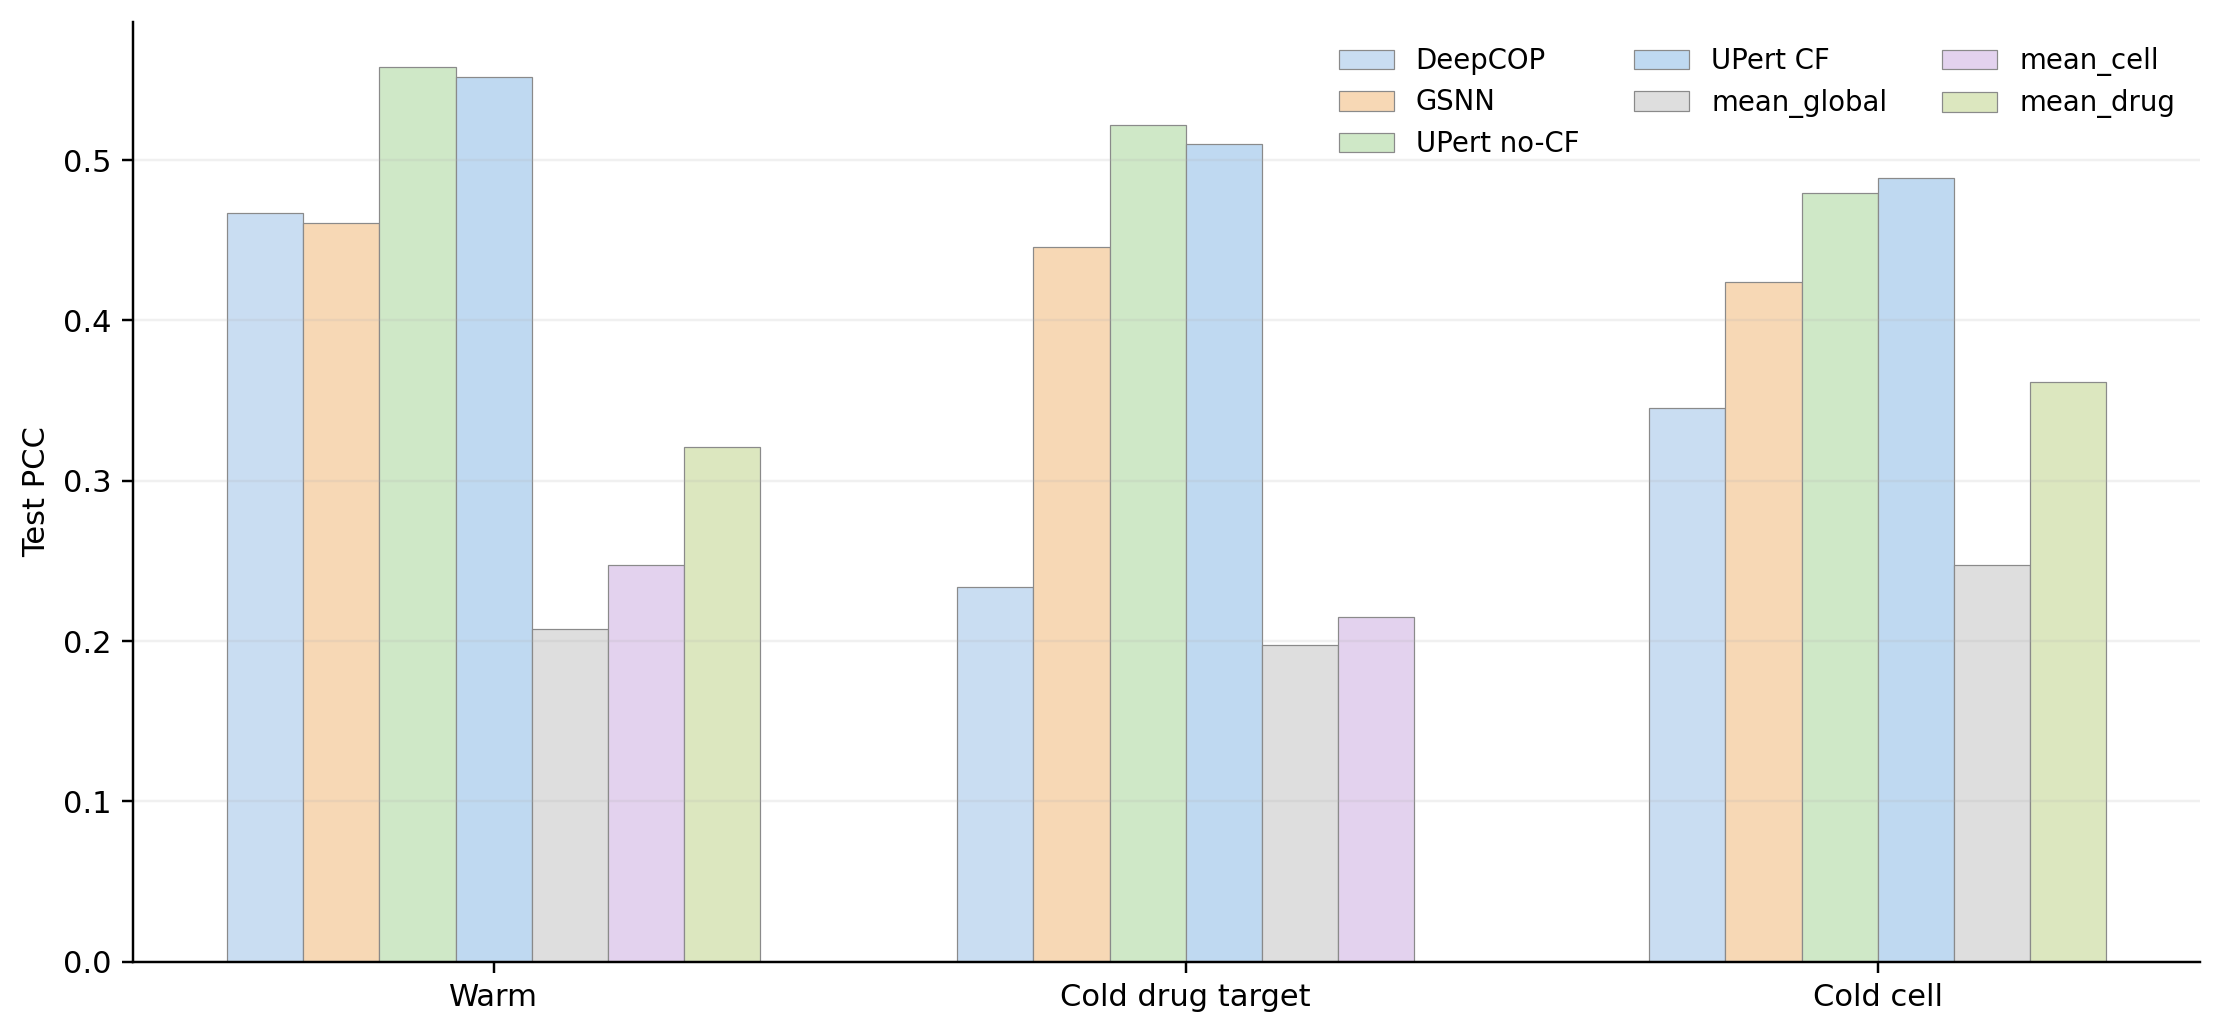
\includegraphics[width=0.86\linewidth]{figures/benchmark_pcc_with_mean_baselines.png}
\caption[PCC with Mean Baselines]{Test PCC in warm, cold drug target, and cold cell for the learned models and the simple mean baselines. mean\_drug is not shown in cold drug target and mean\_cell is not shown in cold cell because these baselines cannot be used there.}
\label{fig:benchmark_pcc_results}
\end{figure}

\subsection{Regulation sign results}
\noindent This metric is used to examine agreement in the direction of change for each gene. The definition of regulation sign accuracy is introduced in the section Evaluation Metrics. Here, the focus is on how the models compare under that metric. The score does not use the response size. It only checks whether the predicted direction of change is correct.

\noindent Table~\ref{tab:sign_accuracy_results} shows the sign agreement results under the three splits. The winner changes with the split. DeepCOP is highest in warm, CAGNN is highest in cold drug target, and GSNN is highest in cold cell. This means the sign metric gives a more mixed ranking than PCC. It also shows that predicting only the direction of change is not exactly the same as predicting the full response shape.

\begin{table}[htbp]
\centering
\caption[Sign Accuracy Across Splits]{Regulation sign accuracy under the three evaluation splits. The best value in each split is shown in bold.}
\label{tab:sign_accuracy_results}
\begin{tabular}{lccc}
\hline
Split & DeepCOP & GSNN & CAGNN \\
\hline
Warm & \textbf{0.6582} & 0.6086 & 0.6496 \\
Cold drug target & 0.5942 & 0.6038 & \textbf{0.6415} \\
Cold cell & 0.5859 & \textbf{0.6084} & 0.5801 \\
\hline
\end{tabular}
\end{table}

\noindent Across the three splits, the lowest PCC values appear in cold cell for all models. The ranking by PCC is also more stable than the ranking by sign accuracy, since CAGNN remains highest in all three splits. The margin is largest in warm and cold drug target and smaller in cold cell.

\subsection{Gene distribution analysis}
\noindent Figure~\ref{fig:xpert_style_gene_distribution} gives a view of model output across selected genes. The figure has three rows, one for each split, and each row shows the distribution of $x_{\mathrm{deg}}$ for twelve genes with strong true response.

\noindent The result is consistent with the summary metrics. In warm and cold drug target, the CAGNN distributions are usually closest to the ground truth distributions across the selected genes. In cold cell, the agreement becomes weaker for all models, but CAGNN still tracks the ground truth more closely than the two baselines in most shown genes.

\begin{figure}[htbp]
\centering
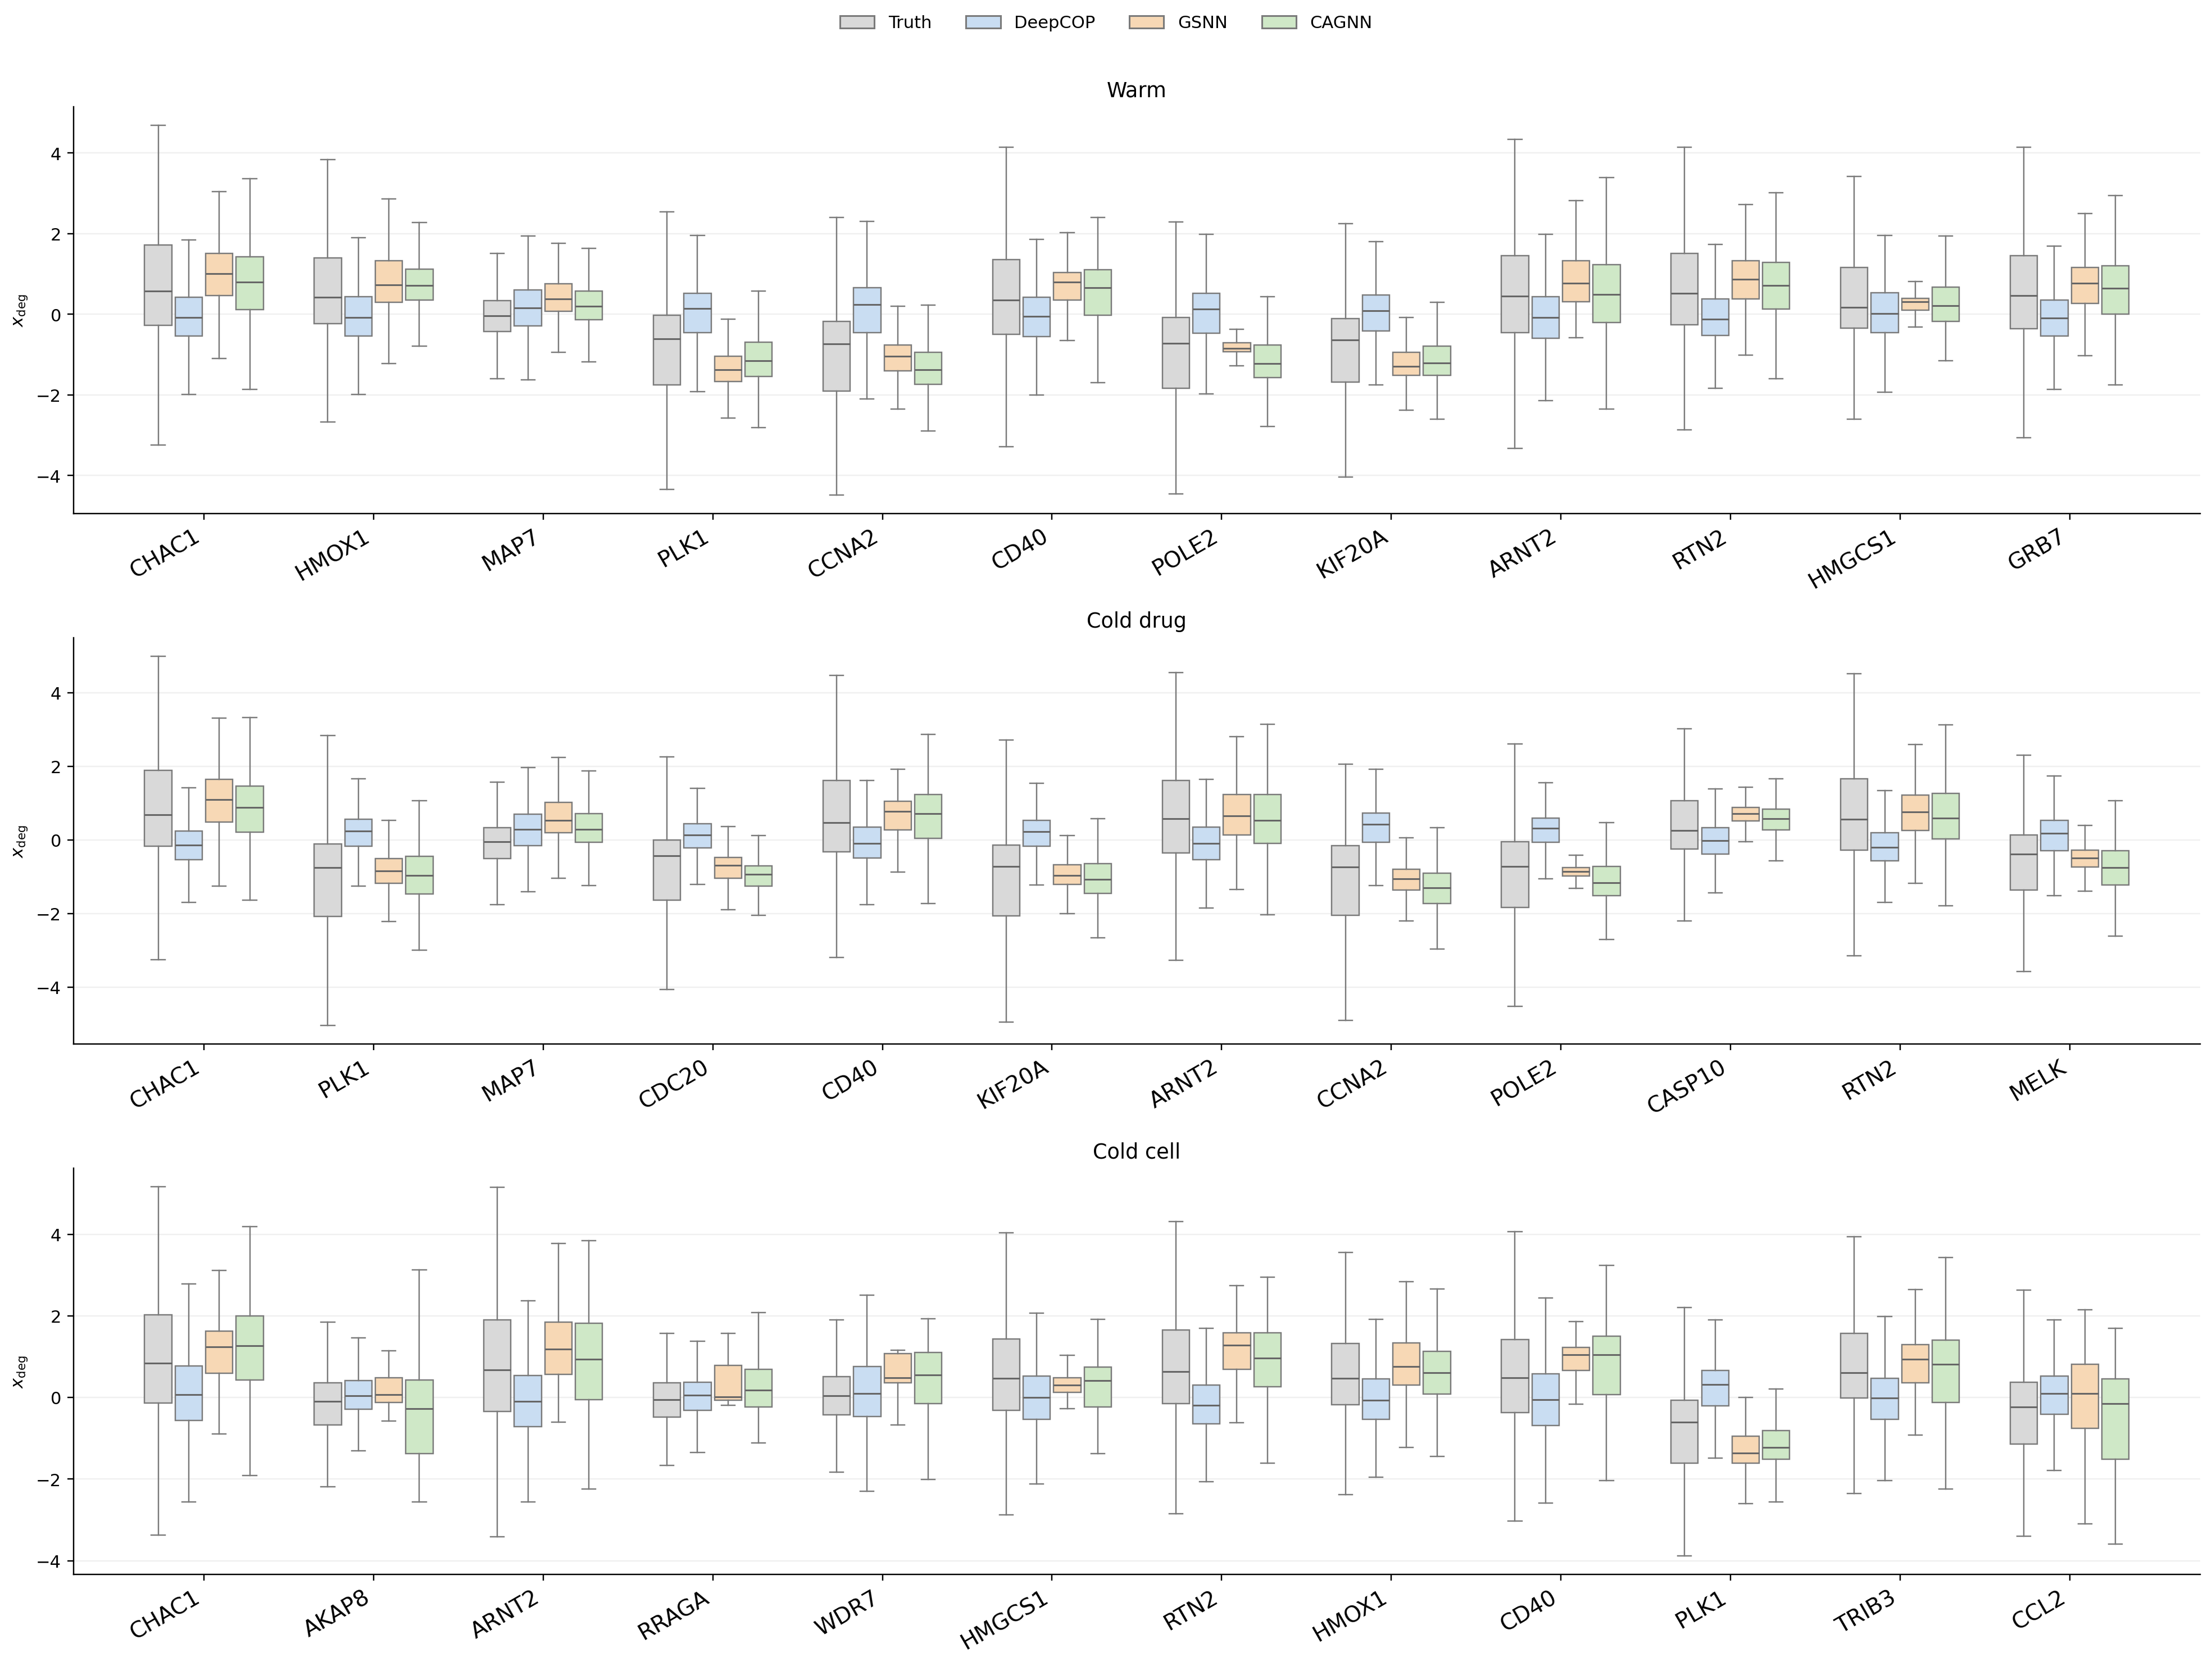
\includegraphics[width=0.98\linewidth]{figures/xpert_style_gene_distribution.png}
\caption[Gene Distribution by Split]{Distribution across selected genes in the three splits. The figure has three rows, one for each split. Each row shows $x_{\mathrm{deg}}$ for twelve genes with strong true response. Ground truth, DeepCOP, GSNN, and CAGNN are shown for each gene.}
\label{fig:xpert_style_gene_distribution}
\end{figure}

\subsection{Ablation analysis}
\noindent This ablation study is separate from the main benchmark comparison. It includes two checks. The first compares two ways of providing cell information to the proposed model. The second tests whether the model still uses the drug input at test time.

\subsubsection{Cell information ablation}
\noindent Table~\ref{tab:context_ablation} shows the results. In the table, ``Cell ID'' means that the model receives only the cell line identity, while ``Control-context'' means that it receives a context vector derived from the matched control profile. Here $\Delta$ means control-context minus Cell ID, so a negative $\Delta$MSE and a positive $\Delta$PCC both indicate improvement. The control-context variant improves both metrics in all three splits. The changes are modest in warm and cold drug target, but much larger in cold cell. The benefit of control-context appears in every split and is strongest when the test cell line is unseen.

\begin{table}[htbp]
\centering
\caption[Cell ID vs Control Context]{Comparison of cell information variants in CAGNN. ``Cell ID'' uses only the cell line identity as input, while ``Control-context'' uses a context vector derived from the matched control profile. The table reports test MSE and test PCC for both variants, together with their differences. Here $\Delta$ means control-context minus Cell ID, so negative $\Delta$MSE and positive $\Delta$PCC indicate improvement.}
\label{tab:context_ablation}
\begin{tabular}{lcccccc}
\hline
Split & Cell ID MSE & Cell ID PCC & Cell-context MSE & Cell-context PCC & $\Delta$MSE & $\Delta$PCC \\
\hline
Warm & 0.8567 & 0.5364 & 0.8218 & 0.5601 & -0.0349 & +0.0237 \\
Cold drug target & 0.9891 & 0.5174 & 0.9542 & 0.5401 & -0.0349 & +0.0227 \\
Cold cell & 1.6983 & 0.3709 & 0.8393 & 0.4778 & -0.8590 & +0.1069 \\
\hline
\end{tabular}
\end{table}

\subsubsection{Drug input sanity check}
\noindent This sanity check asks whether the model still relies on the drug input at test time. The same counterfactual CAGNN model is evaluated twice in each split. The first evaluation uses the normal drug target input, while the second replaces the drug vector with zeros for every test sample. If the model uses drug information, performance should degrade under the zero drug input. Table~\ref{tab:drug_zero_sanity} summarizes the current results. The cold drug target row already uses the latest \texttt{cold\_target\_pattern} result, while warm and cold cell are left as placeholders until the updated runs finish.

\begin{table}[htbp]
\centering
\caption[Zero Drug Sanity Check]{Drug input sanity check for the main counterfactual CAGNN run across the three splits. The standard test setting uses the normal drug target input. The zero drug setting replaces the drug vector with zeros for every test sample. Lower MSE and higher PCC are better.}
\label{tab:drug_zero_sanity}
\begin{tabular}{lcccc}
\hline
Split & Test MSE & Test PCC & Zero drug MSE & Zero drug PCC \\
\hline
Warm & placeholder & placeholder & placeholder & placeholder \\
Cold drug target & 1.3228 & 0.5071 & 1.5575 & 0.4785 \\
Cold cell & placeholder & placeholder & placeholder & placeholder \\
\hline
\end{tabular}
\end{table}

\FloatBarrier
\section{Uncertainty analysis}
In CAGNN, the model predicts both a mean response and a variance term for each gene. The aim here is to examine whether that uncertainty output behaves like a reliability signal. In this section, $\mu$ denotes the predicted mean response, $\sigma^{2}$ denotes the predicted variance, and $\sigma$ is the standard deviation derived from that variance. For probabilistic models, the most direct single quantitative metric is the test negative log likelihood, because it evaluates the predicted mean and variance together under the Gaussian output assumption. Table~\ref{tab:test_nll_results} reports the current test NLL values for warm and cold cell, while the cold drug target entry is left as a placeholder for later completion. The lower NLL in warm than in cold cell is consistent with the view that cold cell is the harder setting. The rest of this section focuses on complementary uncertainty diagnostics through error relations, grouped uncertainty analysis, and coverage of prediction bands. Figure~\ref{fig:uncertainty_summary_placeholder} shows three views of this output, namely uncertainty averaged within each sample, uncertainty versus error, and grouped uncertainty analysis for warm, cold drug target, and cold cell.

\begin{table}[htbp]
\centering
\caption[Test NLL Results]{Test negative log likelihood under the Gaussian output assumption. Lower values are better.}
\label{tab:test_nll_results}
\begin{tabularx}{0.8\textwidth}{lXXX}
\hline
 & Warm & Cold drug target & Cold cell \\
\hline
Test NLL & 0.2812 & placeholder & 0.3170 \\
\hline
\end{tabularx}
\end{table}

\subsection{Uncertainty averaged within each sample}
\noindent Each test sample contains a full vector of predicted gene responses, and each gene also has its own predicted uncertainty. To obtain one simple uncertainty value for the whole sample, the average predicted standard deviation across all genes is used. The left panel of Figure~\ref{fig:uncertainty_summary_placeholder} compares this quantity across the three splits. Warm and cold drug target have similar distributions, while cold cell is shifted slightly upward and shows a somewhat broader upper range.

\subsection{Uncertainty and MSE}
\noindent To check whether the model becomes more uncertain when it makes larger mistakes, each test sample is plotted by its uncertainty averaged within that sample and its MSE for that sample. In all three splits, the point clouds show a positive relationship. The trend is strongest in cold cell, moderate in warm, and weaker in cold drug target. When reading the middle upper panel of Figure~\ref{fig:uncertainty_summary_placeholder}, the key pattern is that higher uncertainty values are usually associated with higher MSE.

\subsection{Uncertainty and PCC}
\noindent A related analysis compares the same uncertainty value with PCC computed separately for each sample. This gives a different view from MSE. In Figure~\ref{fig:uncertainty_summary_placeholder}, only cold cell shows a clearly visible negative relationship. In warm and cold drug target, the relationship between uncertainty and PCC is much weaker. The uncertainty output therefore follows absolute error more clearly than correlation measured within each sample.

\subsection{Uncertainty groups analysis}
\noindent The same pattern can be shown more directly by grouping test samples into low, medium, and high uncertainty groups. The groups are formed by sorting the samples according to the uncertainty averaged within each sample and splitting them into three equal sized parts. The average MSE and PCC are then calculated inside each group. In the right panel of Figure~\ref{fig:uncertainty_summary_placeholder}, the main pattern is clear for MSE in all three splits, since the high uncertainty group always has the largest mean error. For PCC, the separation is visible mainly in cold cell and much weaker in warm and cold drug target.

\begin{figure}[htbp]
\centering
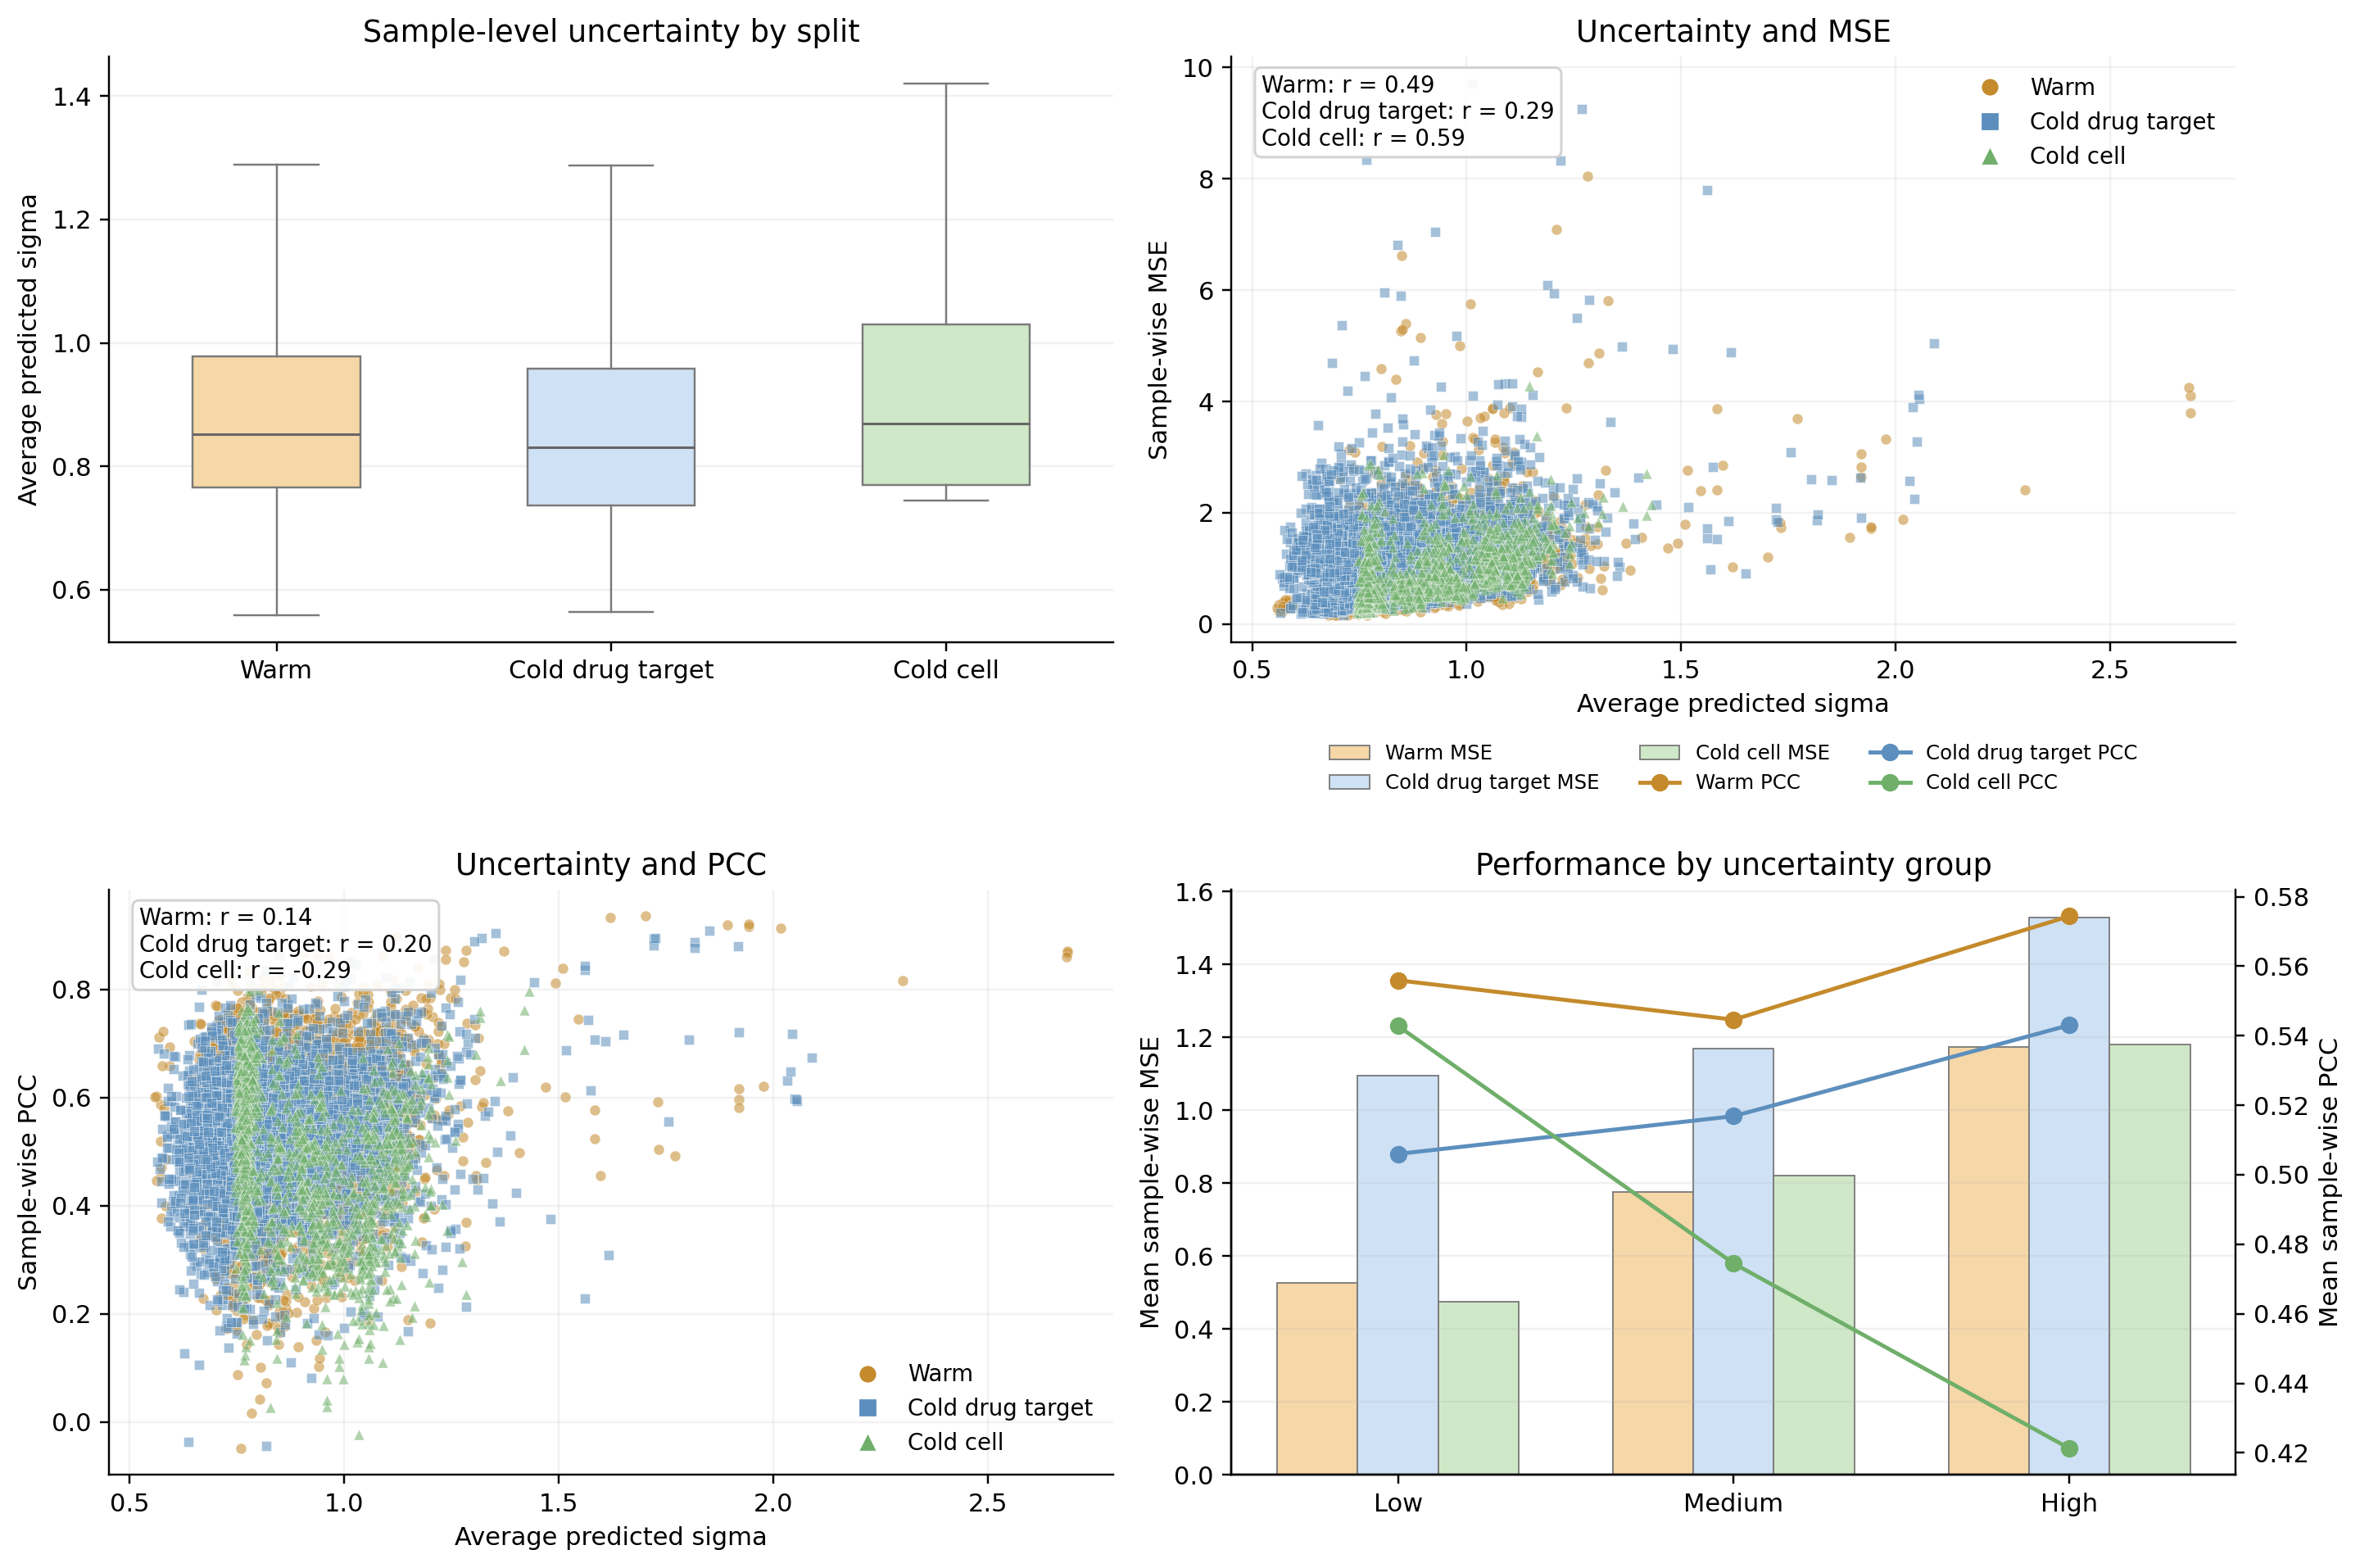
\includegraphics[width=0.98\linewidth]{figures/uncertainty_summary_placeholder.png}
\caption[Uncertainty Summary]{Uncertainty summary in warm, cold drug target, and cold cell, based on the test set. The left panel shows uncertainty averaged within each sample in the three splits. The middle panels compare uncertainty with MSE and PCC. The right panel shows MSE and PCC for low, medium, and high uncertainty groups in each split.}
\label{fig:uncertainty_summary_placeholder}
\end{figure}

\noindent Figure~\ref{fig:uncertainty_summary_placeholder} highlights three consistent observations. Cold cell is slightly more uncertain overall. Uncertainty is more clearly related to MSE than to PCC. High uncertainty groups also have larger MSE in all three splits.

\subsection{Coverage of prediction bands}
\noindent Under a Gaussian interpretation, the band $\mu \pm 2\sigma$ can be read as an approximate 95\% prediction interval. To check this more directly, the empirical coverage is calculated on the full test set as the fraction of target genes whose true values fall inside $\mu \pm 2\sigma$. Table~\ref{tab:uncertainty_empirical_coverage} shows that the coverage is close to 95\% in all three splits. This is useful as a calibration style diagnostic, but it does not replace a full likelihood based evaluation such as test NLL.

\begin{table}[htbp]
\centering
\caption[Prediction Band Coverage]{Coverage of the prediction band $\mu \pm 2\sigma$ on the full test set.}
\label{tab:uncertainty_empirical_coverage}
\begin{tabularx}{0.8\textwidth}{lXXX}
\hline
 & Warm & Cold drug target & Cold cell \\
\hline
Coverage & 95.96\% & 94.00\% & 96.30\% \\
\hline
\end{tabularx}
\end{table}

\subsection{Uncertainty across genes}
\noindent The uncertainty output can also be studied across genes instead of across samples. For each gene, the predicted standard deviation is averaged across all test samples. This makes it possible to identify genes that are repeatedly assigned higher uncertainty and to compare uncertainty across genes with prediction error across genes. Figure~\ref{fig:gene_level_uncertainty_warm} shows this view.

\noindent The left panel shows the genes with the highest mean predicted $\sigma$. The right panel compares mean $\sigma$ across genes with MSE across genes. The relationship is again positive, since genes with larger mean uncertainty also tend to have larger MSE.

\begin{figure}[htbp]
\centering
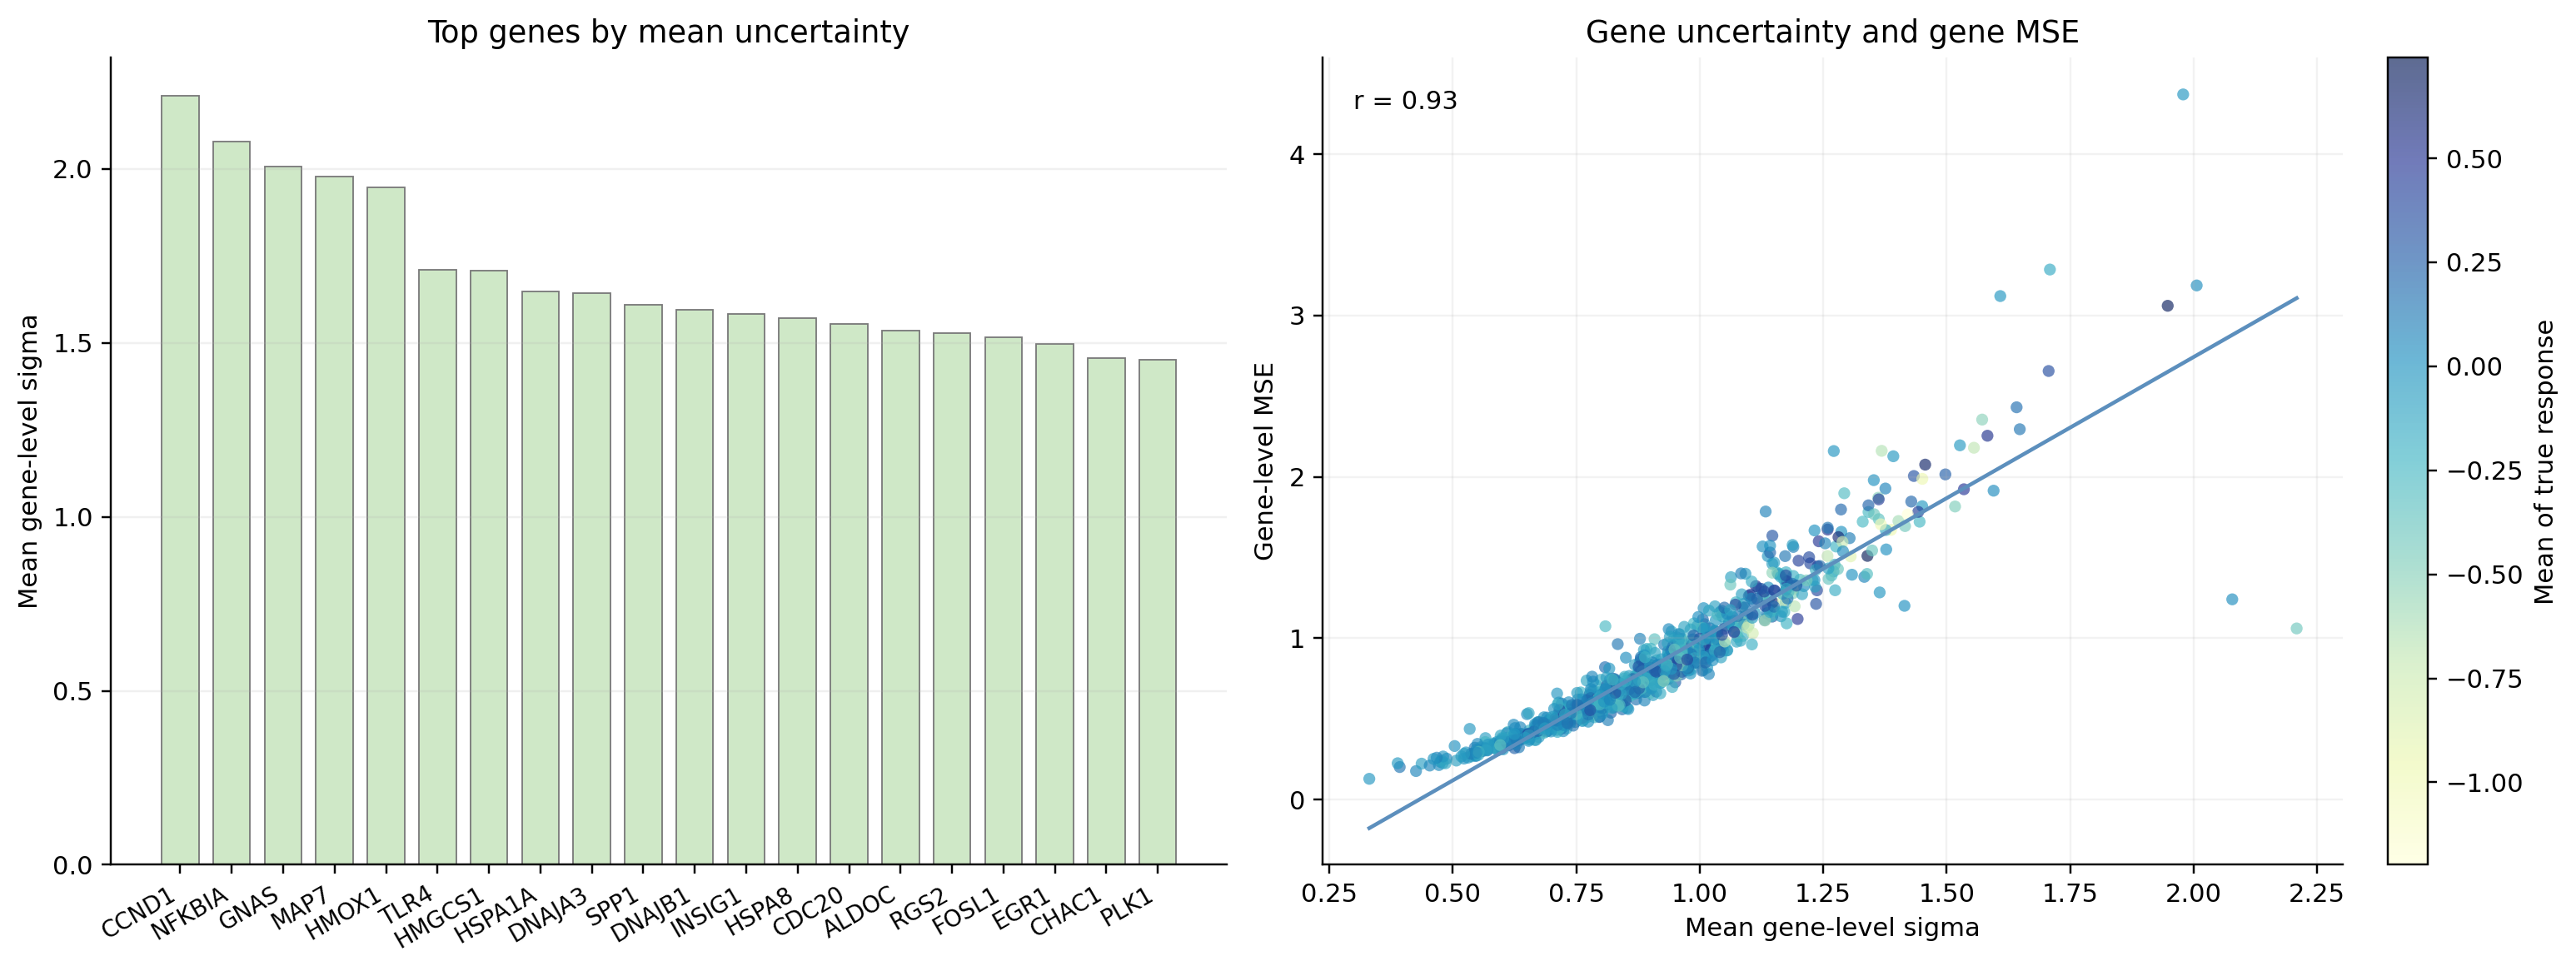
\includegraphics[width=0.98\linewidth]{figures/gene_level_uncertainty_warm.png}
\caption[Gene Uncertainty]{The left panel shows the top 20 genes with the highest mean predicted standard deviation on the test set. The right panel compares mean $\sigma$ across genes with MSE across genes for all target genes on the test set.}
\label{fig:gene_level_uncertainty_warm}
\end{figure}

\subsection{Case studies with mean and uncertainty}
\noindent The uncertainty output can also be inspected in individual examples. In Figure~\ref{fig:uncertainty_case_placeholder}, each panel shows one test sample. The plot includes the true response, the predicted mean, and the prediction band $\mu \pm 2\sigma$. Table~\ref{tab:uncertainty_empirical_coverage} already shows that this band gives close to 95\% coverage on the full test set. To keep the figure readable, each panel shows only the twelve genes with the largest absolute true response in that sample. The selection is based on $y_{\mathrm{true}}$, not on $y_{\mathrm{pred}}$. For each split, the left panel shows a lower uncertainty sample with a better fit, while the right panel shows a higher uncertainty sample with a larger error. These displayed cases are only visual examples, so their local coverage can differ from the full test set coverage.

\begin{figure}[htbp]
\centering
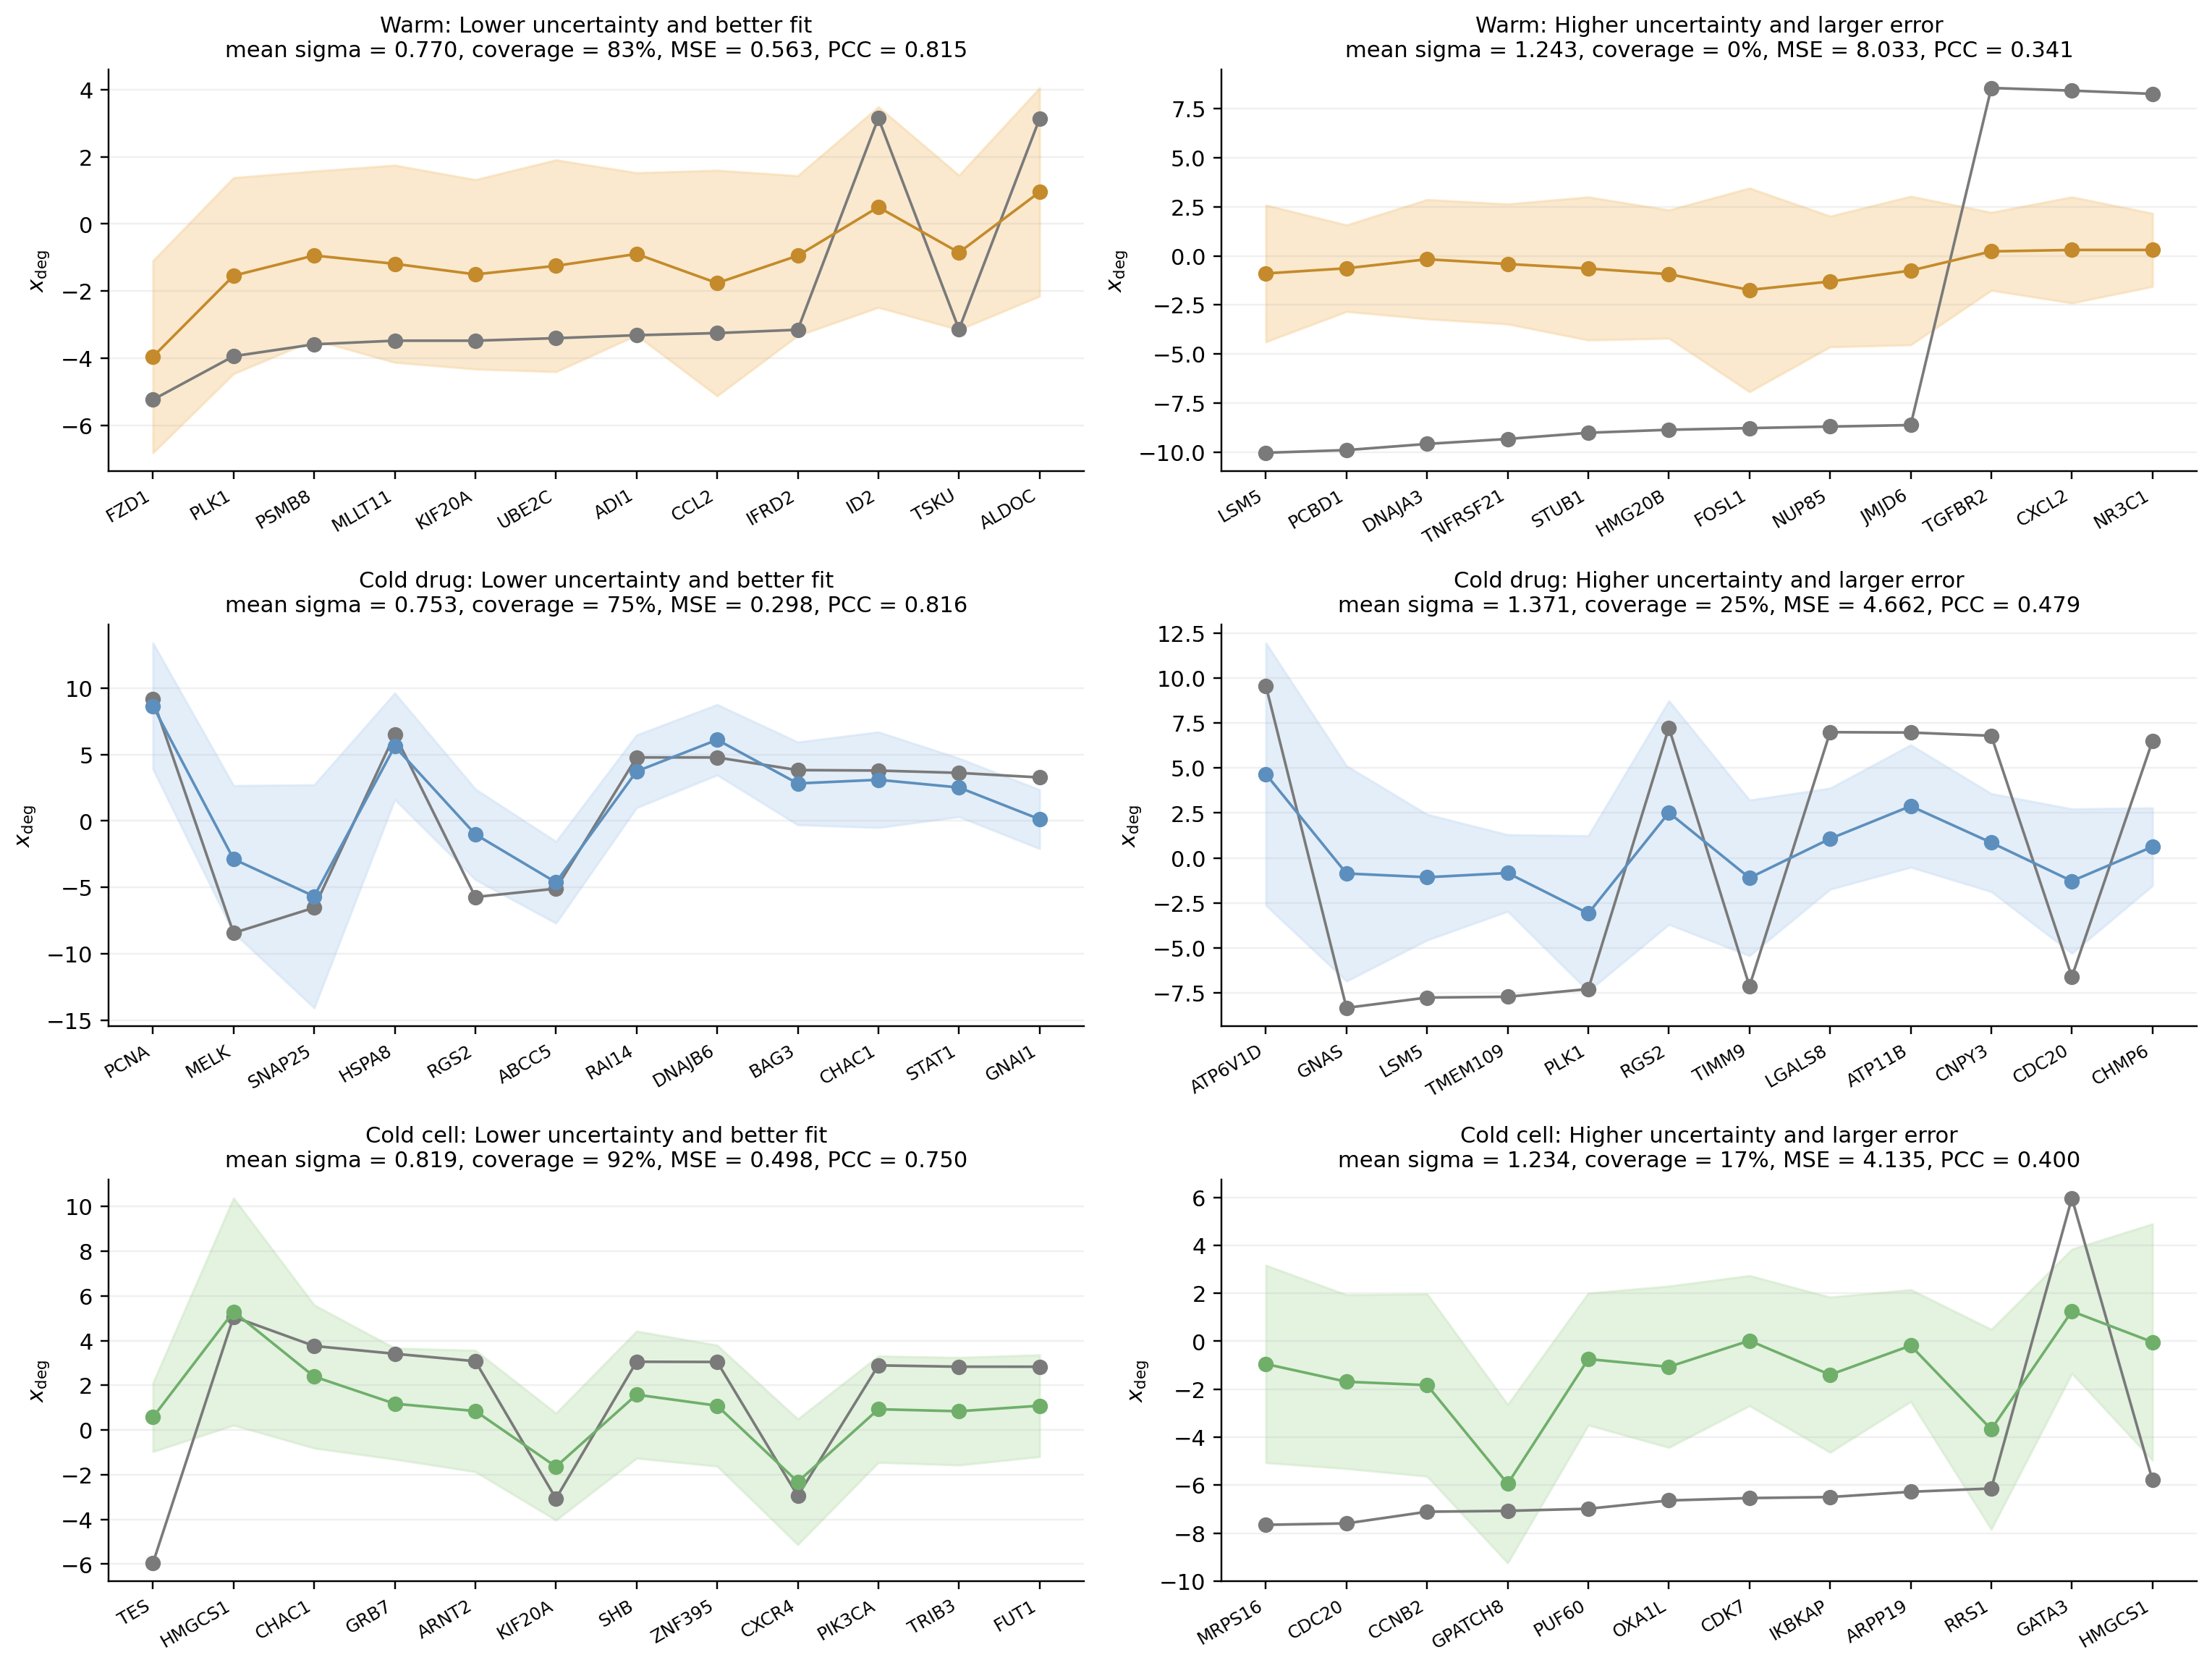
\includegraphics[width=0.98\linewidth]{figures/uncertainty_case_study_placeholder.png}
\caption[Uncertainty Case Studies]{Case studies with uncertainty bands in warm, cold drug target, and cold cell. In each split, the left panel shows a lower uncertainty sample with a better fit, and the right panel shows a higher uncertainty sample with a larger error. Each panel uses the twelve genes with the largest absolute true response in that sample. The plots show the true response, the predicted mean, and the prediction band $\mu \pm 2\sigma$.}
\label{fig:uncertainty_case_placeholder}
\end{figure}
\FloatBarrier
\section{Data efficiency evaluation}
This part examines how model performance changes as the amount of training data increases in the warm split. Only the warm split is used here, because the goal is to study the effect of training budget itself. In cold drug target and cold cell, performance is also affected by unseen drugs or unseen cell lines, so the effect of less training data would be harder to interpret. It is a separate budget analysis rather than another three split benchmark table. The detailed setup is introduced in the methodology chapter. Figure~\ref{fig:data_efficiency_placeholder} shows how the models improve as more training samples are available.

\begin{figure}[htbp]
\centering
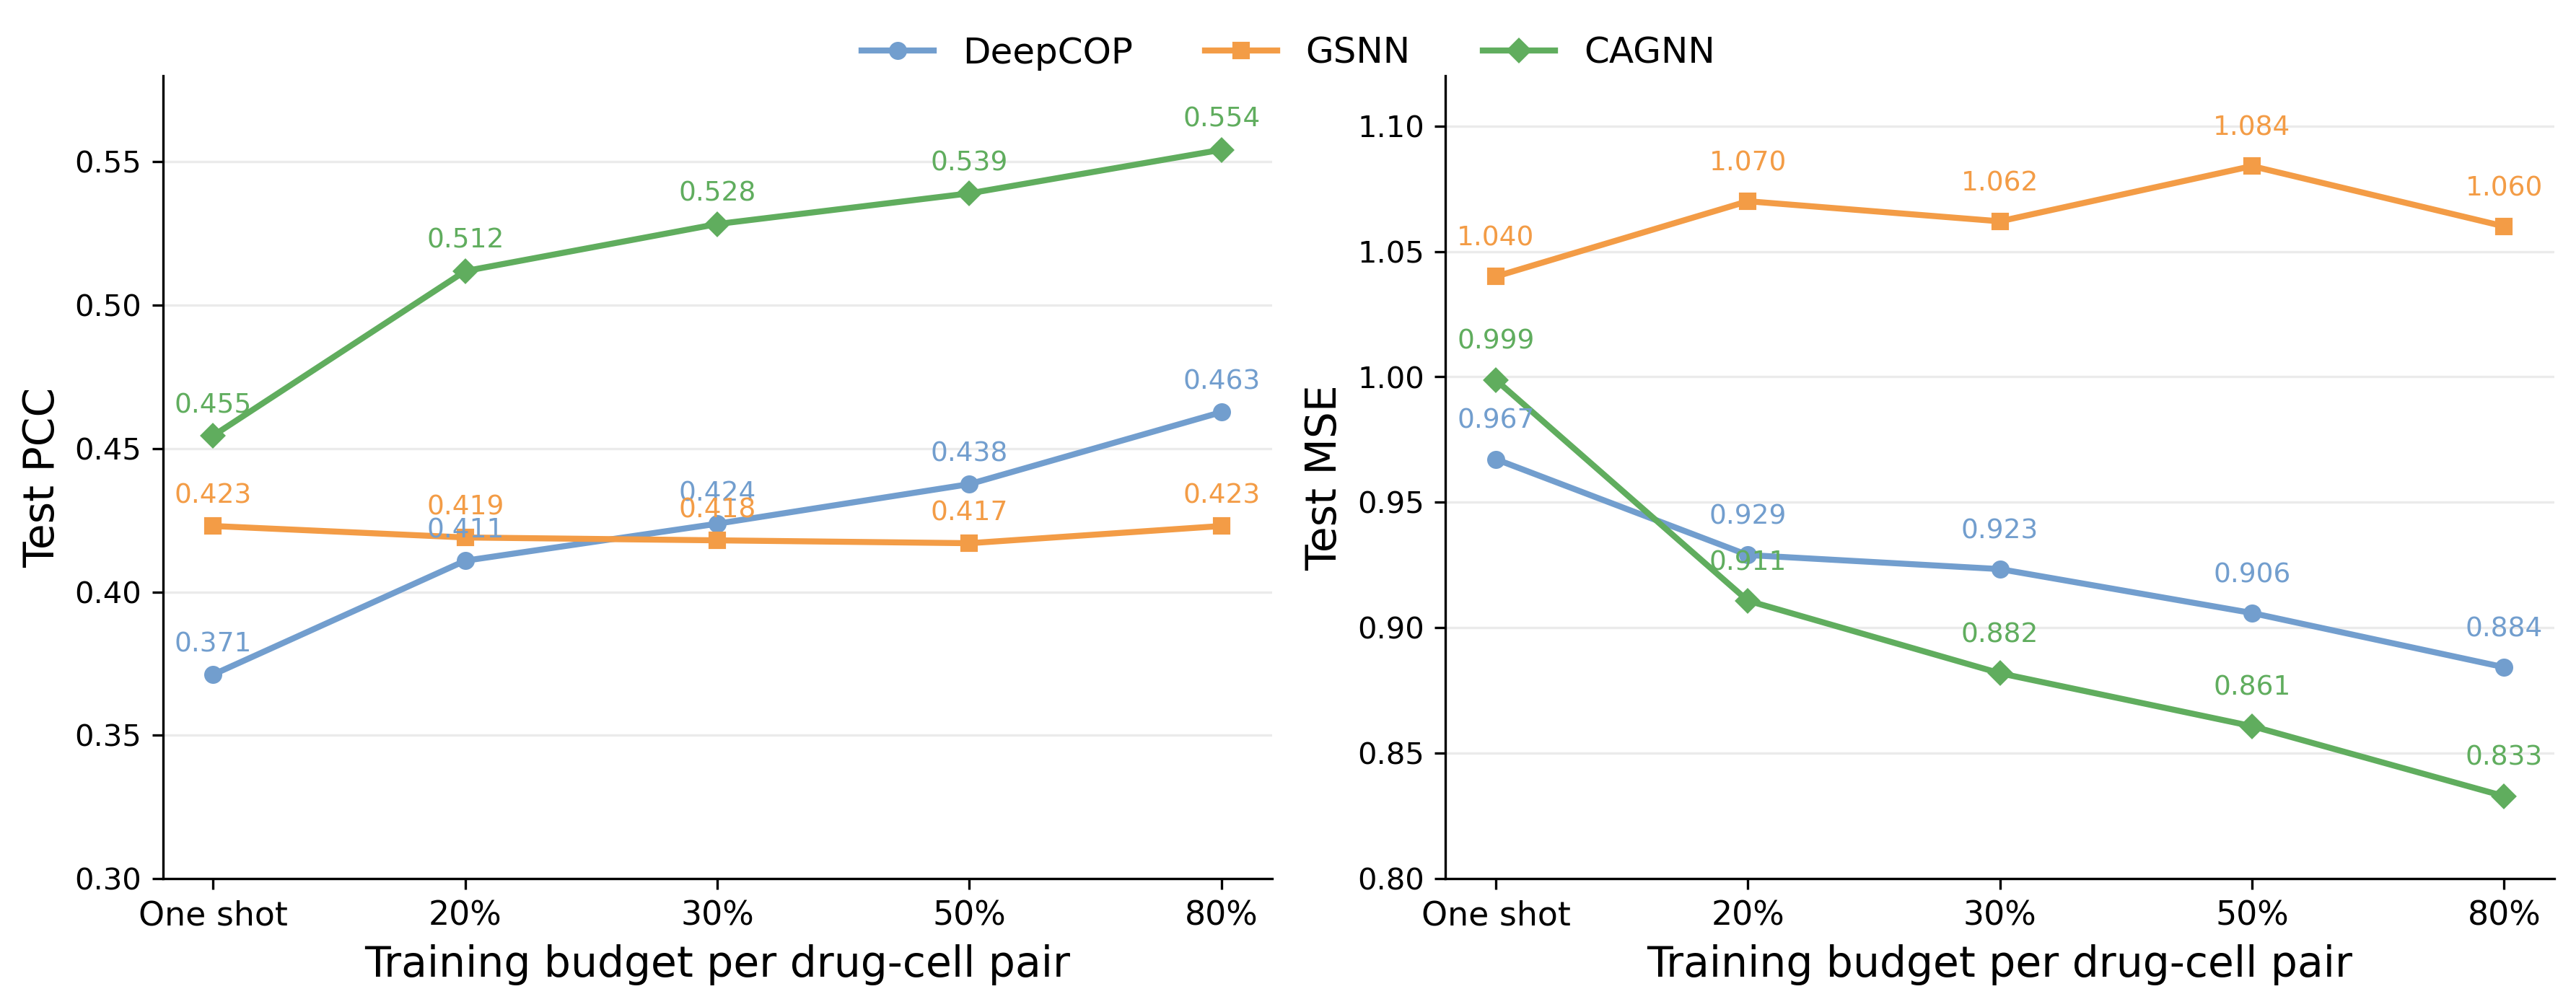
\includegraphics[width=0.94\linewidth]{figures/data_efficiency_warm_real.png}
\caption[Warm Data Efficiency]{Warm split data efficiency results. The left panel shows test PCC and the right panel shows test MSE for DeepCOP, GSNN, and CAGNN across the displayed training budgets. In the updated DeepCOP budget runs, DeepCOP also improves clearly as more training data are used, while GSNN changes less across the same budgets.}
\label{fig:data_efficiency_placeholder}
\end{figure}

\noindent Figure~\ref{fig:data_efficiency_placeholder} shows that CAGNN remains strongest on PCC across the displayed warm split budgets, and its advantage is already visible at smaller budgets. In the updated DeepCOP budget runs, DeepCOP also improves steadily as more data are added, with higher PCC and lower MSE across the shown budgets. GSNN changes less over the same range.
\FloatBarrier
\section{Interpretation and case studies}
\noindent Average metrics show overall performance, but they do not show how the model uses the graph in one specific example. The following cases are selected from CAGNN. Here attention means the weight that the model gives to one graph edge during message passing. A larger weight means that the model uses that edge more strongly in the final prediction. These weights are not treated as proof of a real biological mechanism. The analysis instead asks two simple questions. Are the highly weighted edges easier to understand when the prediction is accurate, and does the model keep giving high weights to similar edges across different settings.

\noindent Table~\ref{tab:case_study_terms} gives short explanations of the main biology terms used in this section. These short notes are only meant to help reading. They do not replace the full biological background of each gene or drug class.

\begin{table}[htbp]
\centering
\caption[Biology Terms for Case Studies]{Short explanations of selected biology terms used in the attention analysis and case studies.}
\label{tab:case_study_terms}
\begin{tabular}{p{3.0cm}p{10.0cm}}
\hline
Term & Simple meaning \\
\hline
\texttt{SB-939} & A drug in the case study. It is reported as an HDAC inhibitor. \\
\texttt{CAY-10585} & A drug in the case study. It is reported as a \texttt{HIF modulator}. \\
\texttt{alvocidib} & A drug in the case study. It is reported as a \texttt{CDK inhibitor}. \\
\texttt{HDAC inhibitor} & A drug class that acts on proteins that help control which genes are turned on or off. \\
\texttt{HIF1A} & A transcription factor related to hypoxia response, metabolic adaptation, and stress signaling. \\
\texttt{CDK inhibitor} & A drug class that acts on proteins involved in cell division. \\
\texttt{BCL2 family proteins} & Proteins involved in whether a cell survives or dies. \\
\texttt{TP53} & A broad stress and damage response regulator. It is often active when the cell is under pressure or has been damaged. \\
\texttt{NR3C1} & A regulator related to stress response and cell state. \\
\hline
\end{tabular}
\end{table}

\noindent For the cold drug target analysis, the case studies are taken from the \texttt{cold\_target\_pattern} split. In this split, the held out test drugs do not share target genes or target patterns with the training drugs. The attention analysis therefore asks whether the model still gives readable high weight edges when the drug target information is fully unseen during training. The attention tables below use the main counterfactual CAGNN run. In the same split, the no counterfactual variant gives slightly better summary metrics, with test MSE $1.2645$ and test PCC $0.5218$, compared with test MSE $1.3228$ and test PCC $0.5071$ for the counterfactual run. The two examples shown here are \texttt{BRD-K86797399} and \texttt{BRD-K88551539}, chosen directly from the current exported attention results for this split.

\noindent Figure~\ref{fig:best_drug_top20_heatmap} and Figure~\ref{fig:worst_drug_top20_heatmap} show where the model places the largest edge weights for the 20 best and 20 worst predicted drugs. Each figure highlights the strongest connections. This gives a view of whether the model keeps its focus on a smaller set of edges or spreads the weight across many edges.

\begin{figure}[htbp]
\centering
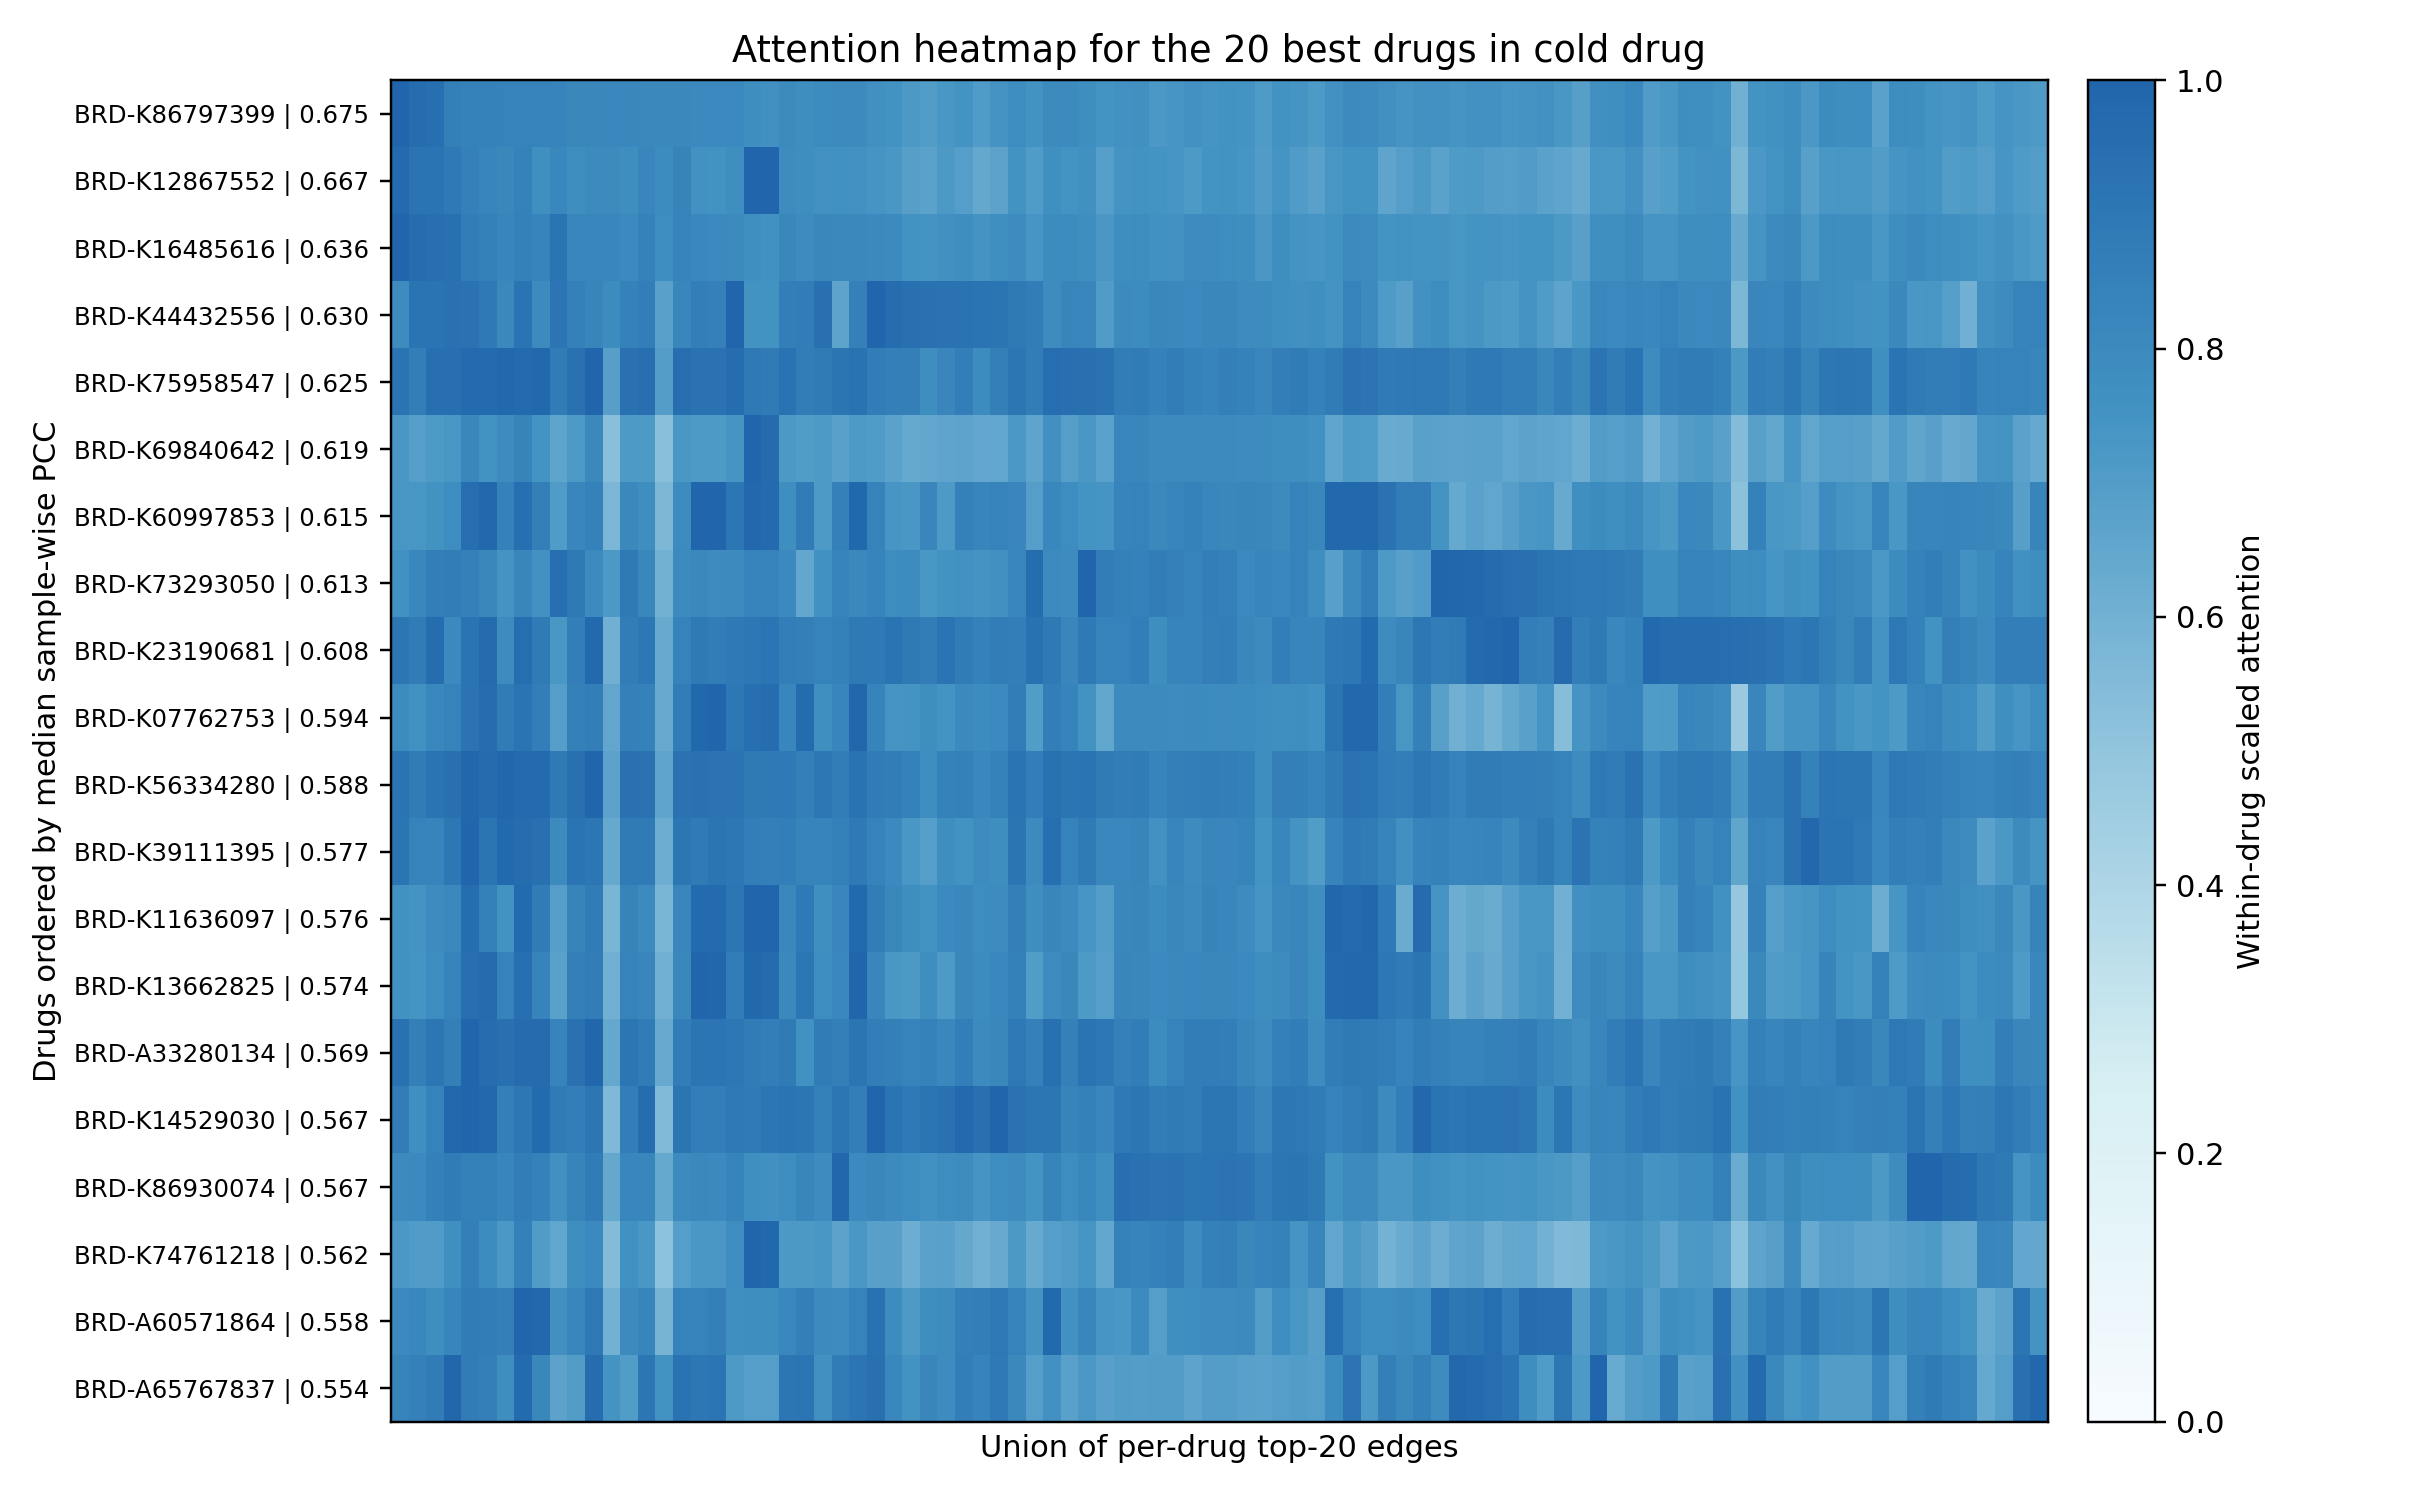
\includegraphics[width=\linewidth]{figures/attention_best_drugs_top20_heatmap.png}
\caption[Best Cold Drug Target Heatmap]{Attention heatmap for the top 20 best drugs in the cold drug target split. For each drug, the heatmap shows the strongest edges between different genes. The values are scaled within each drug. Darker blue regions show where the model puts more attention.}
\label{fig:best_drug_top20_heatmap}
\end{figure}

\begin{figure}[htbp]
\centering
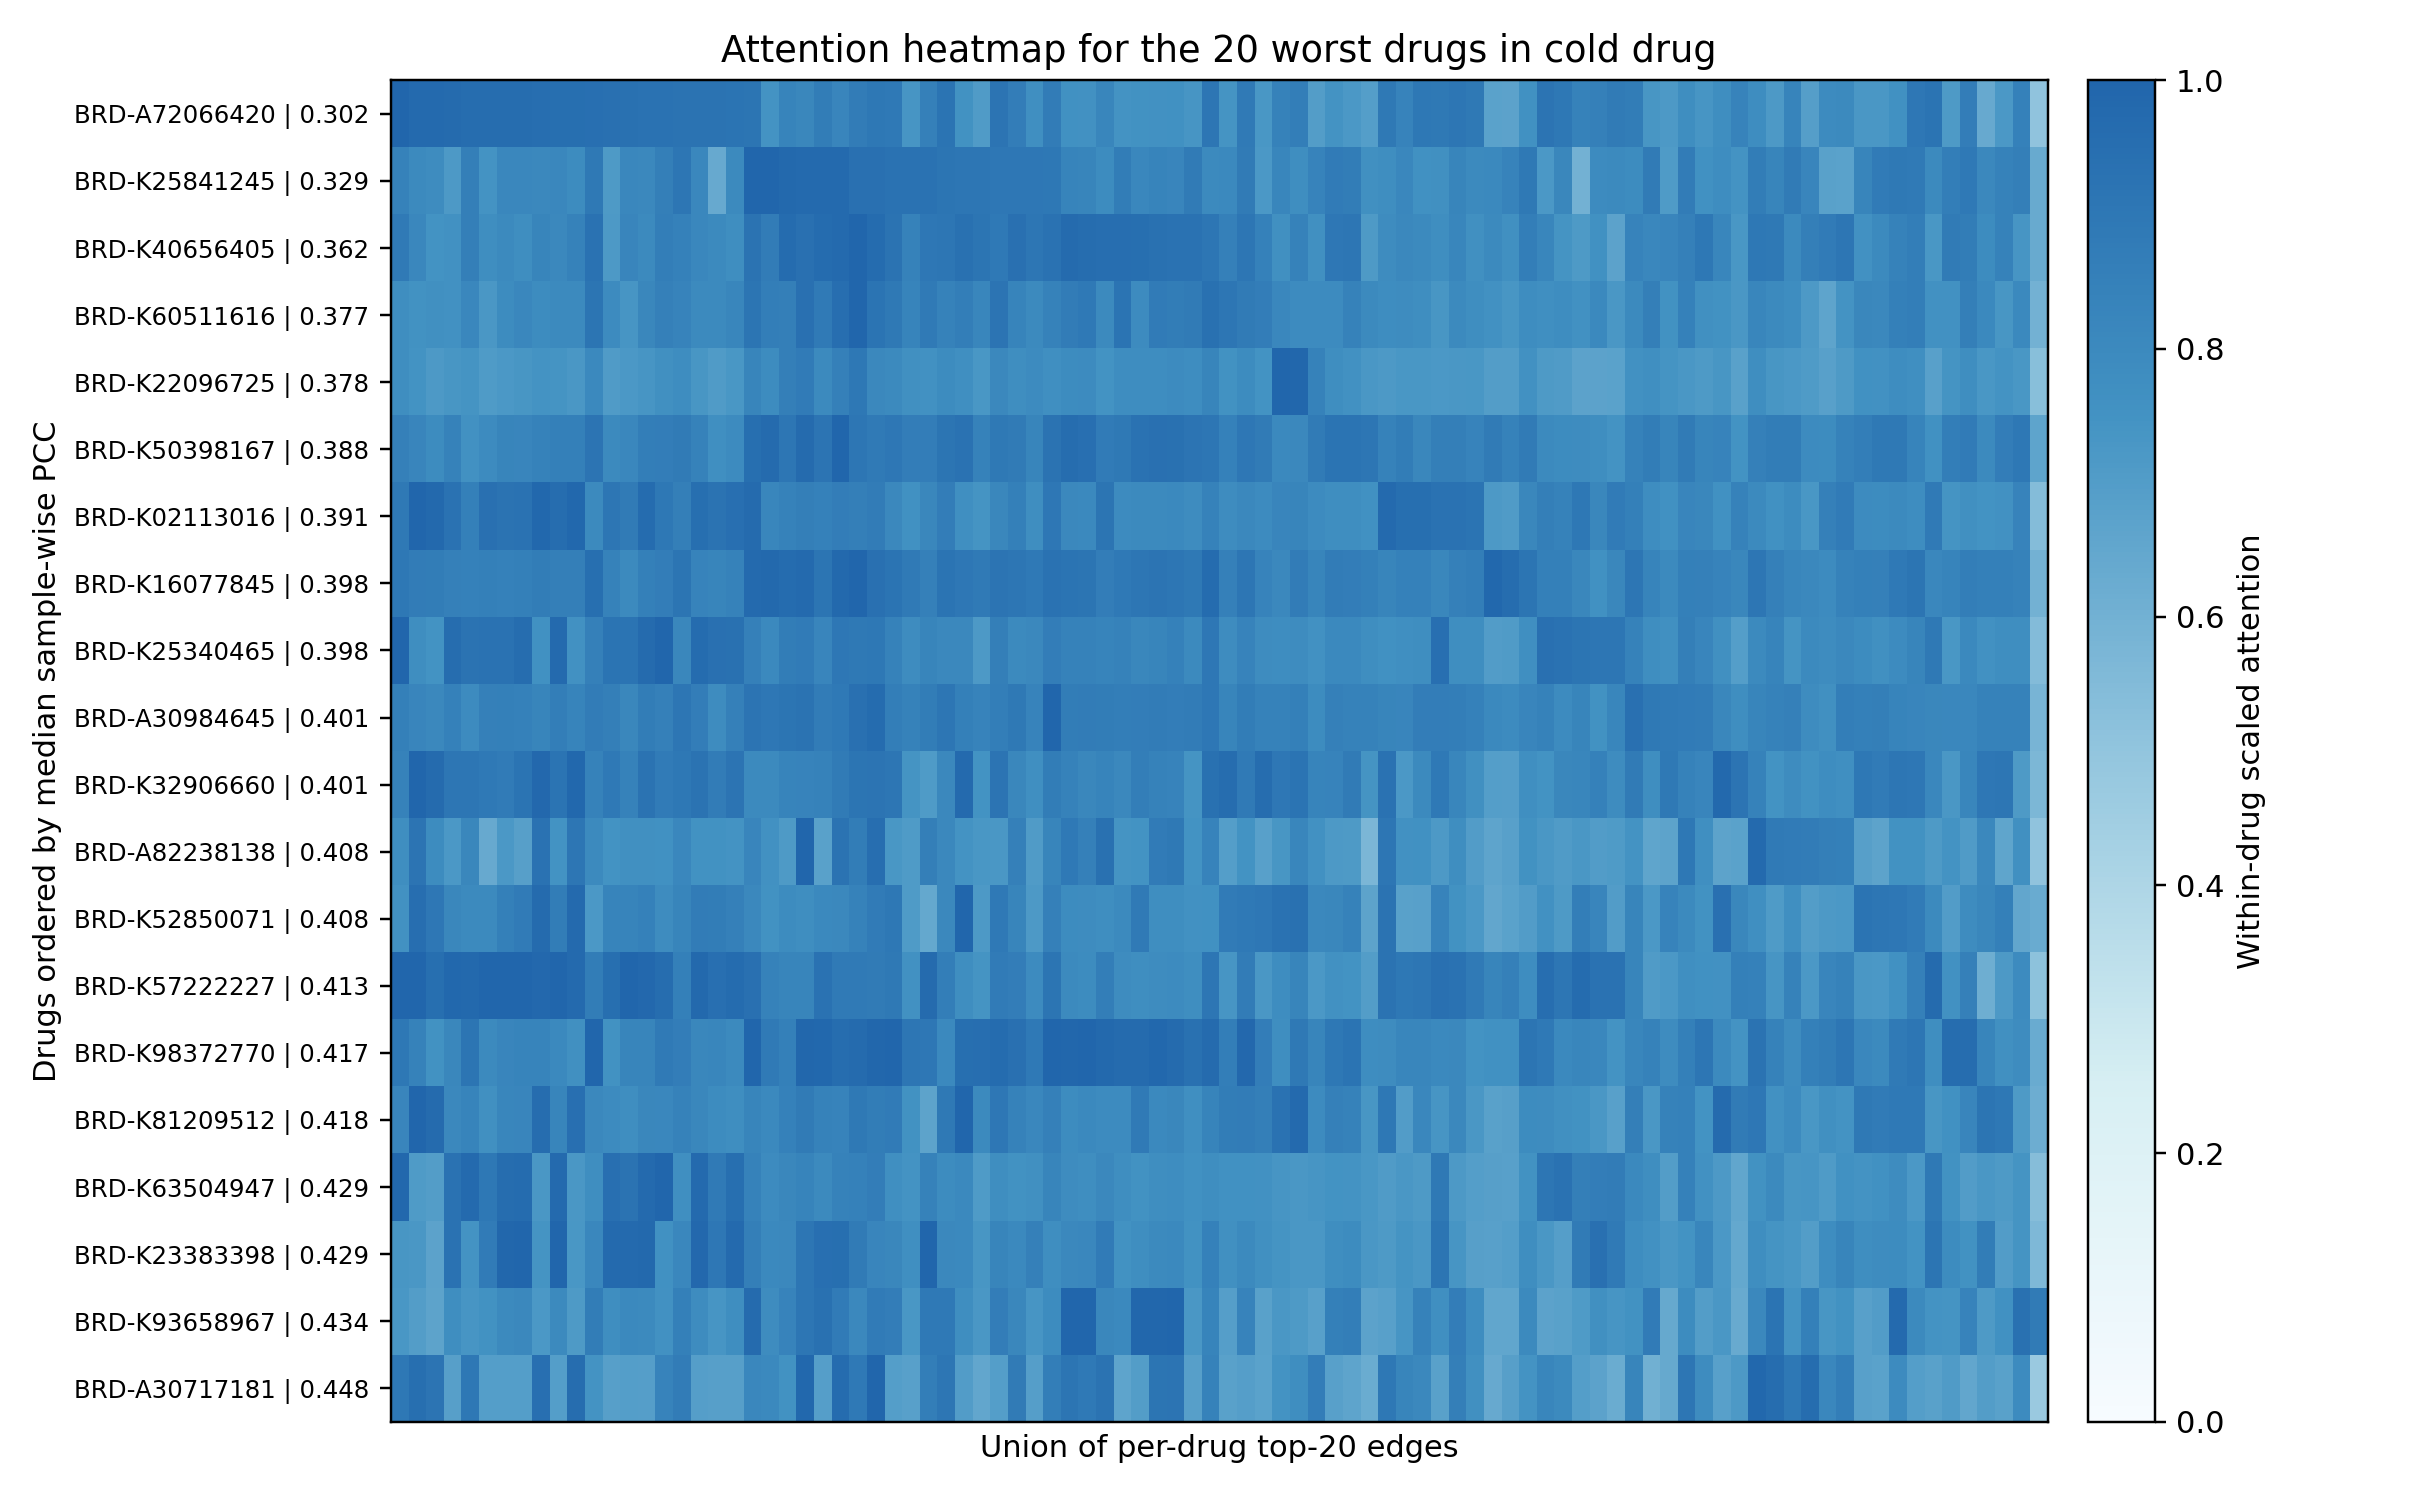
\includegraphics[width=\linewidth]{figures/attention_worst_drugs_top20_heatmap.png}
\caption[Worst Cold Drug Target Heatmap]{Attention heatmap for the top 20 worst drugs in the cold drug target split. For each drug, the heatmap shows the strongest edges between different genes. The values are adjusted within each drug. Darker blue regions show where the model puts more attention.}
\label{fig:worst_drug_top20_heatmap}
\end{figure}

\noindent These two heatmaps give an overview before looking at individual drugs. In the best predicted cases, darker values often appear in a smaller and more repeated set of edges. In the worst predicted cases, the weights are spread more widely. But weak predictions can still contain large edge weights. For that reason, the heatmaps alone are not enough, and the edge lists in Table~\ref{tab:attention_cold_drug_target_best_worst} are needed for closer reading.

\noindent Among the selected cold drug target examples, SB-939, labeled as \texttt{BRD-K86797399}, provides one representative case. This compound is reported as an \texttt{HDAC inhibitor}. In the current exported attention file, its top edges include \texttt{HIF1A}$\rightarrow$\texttt{KDM3A}, \texttt{HIF1A}$\rightarrow$\texttt{ALDOA}, and \texttt{HIF1A}$\rightarrow$\texttt{BNIP3}. These edges still point to a readable stress and metabolic response neighborhood, even though the known drug targets themselves are HDAC family proteins rather than \texttt{HIF1A}.

\noindent The second example is CAY-10585, labeled as \texttt{BRD-K88551539}, which is reported as a \texttt{HIF modulator} with target \texttt{HIF1A}. Here the attention pattern is easier to connect to the reported mechanism. The top edges include \texttt{HIF1A}$\rightarrow$\texttt{KDM3A}, \texttt{HIF1A}$\rightarrow$\texttt{S100A4}, \texttt{HIF1A}$\rightarrow$\texttt{ALDOA}, and \texttt{HIF1A}$\rightarrow$\texttt{BNIP3}. This is useful because \texttt{ALDOA} and \texttt{BNIP3} are well known hypoxia related downstream genes, so the attention map is easier to read as a target centered response program.

\begin{table}[htbp]
\centering
\caption[Cold Drug Target Case Edges]{Top high attention edges for two illustrative cold drug target examples from the main counterfactual CAGNN run. The left columns show \texttt{BRD-K86797399}, and the right columns show \texttt{BRD-K88551539}. Attention values come from the last attention layer.}
\label{tab:attention_cold_drug_target_best_worst}
\begin{tabular}{lclc}
\hline
SB-939 edge & Attention & CAY-10585 edge & Attention \\
\hline
\texttt{PCNA}$\rightarrow$\texttt{POLD4} & 0.6428 & \texttt{HIF1A}$\rightarrow$\texttt{KDM3A} & 0.6222 \\
\texttt{HIF1A}$\rightarrow$\texttt{KDM3A} & 0.6419 & \texttt{HIF1A}$\rightarrow$\texttt{S100A4} & 0.6107 \\
\texttt{HIF1A}$\rightarrow$\texttt{ALDOA} & 0.6160 & \texttt{PCNA}$\rightarrow$\texttt{POLD4} & 0.6097 \\
\texttt{HIF1A}$\rightarrow$\texttt{SLC11A2} & 0.6150 & \texttt{AKT1}$\rightarrow$\texttt{HK1} & 0.5968 \\
\texttt{HIF1A}$\rightarrow$\texttt{BNIP3} & 0.5970 & \texttt{AKT1}$\rightarrow$\texttt{USP14} & 0.5812 \\
\texttt{E2F2}$\rightarrow$\texttt{EED} & 0.5890 & \texttt{HIF1A}$\rightarrow$\texttt{ALDOA} & 0.5803 \\
\texttt{CDK1}$\rightarrow$\texttt{RNMT} & 0.5846 & \texttt{HIF1A}$\rightarrow$\texttt{SLC11A2} & 0.5760 \\
\texttt{GATA2}$\rightarrow$\texttt{MAPKAPK3} & 0.5747 & \texttt{HIF1A}$\rightarrow$\texttt{BNIP3} & 0.5647 \\
\texttt{HMGA2}$\rightarrow$\texttt{IGF2BP2} & 0.5702 & \texttt{E2F2}$\rightarrow$\texttt{EED} & 0.5599 \\
\texttt{CDK1}$\rightarrow$\texttt{USP1} & 0.5686 & \texttt{HMGA2}$\rightarrow$\texttt{IGF2BP2} & 0.5598 \\
\hline
\end{tabular}
\end{table}

\noindent Table~\ref{tab:attention_cold_drug_target_best_worst} makes this comparison clearer. The main difference is not simply the size of the edge weights. The more useful question is whether the highlighted edges can be summarized in a readable way that matches the reported drug target and a plausible downstream response program. Attention should therefore be read together with prediction quality and prior biological knowledge, not on its own.

\noindent The cold cell test asks a different question. Instead of comparing different drugs, it asks whether the same drug keeps a readable set of high weight edges when the cell line is unseen. Figure~\ref{fig:best_drug_top20_heatmap_cold_cell} shows the top 20 best drugs in this setting.

\begin{figure}[htbp]
\centering
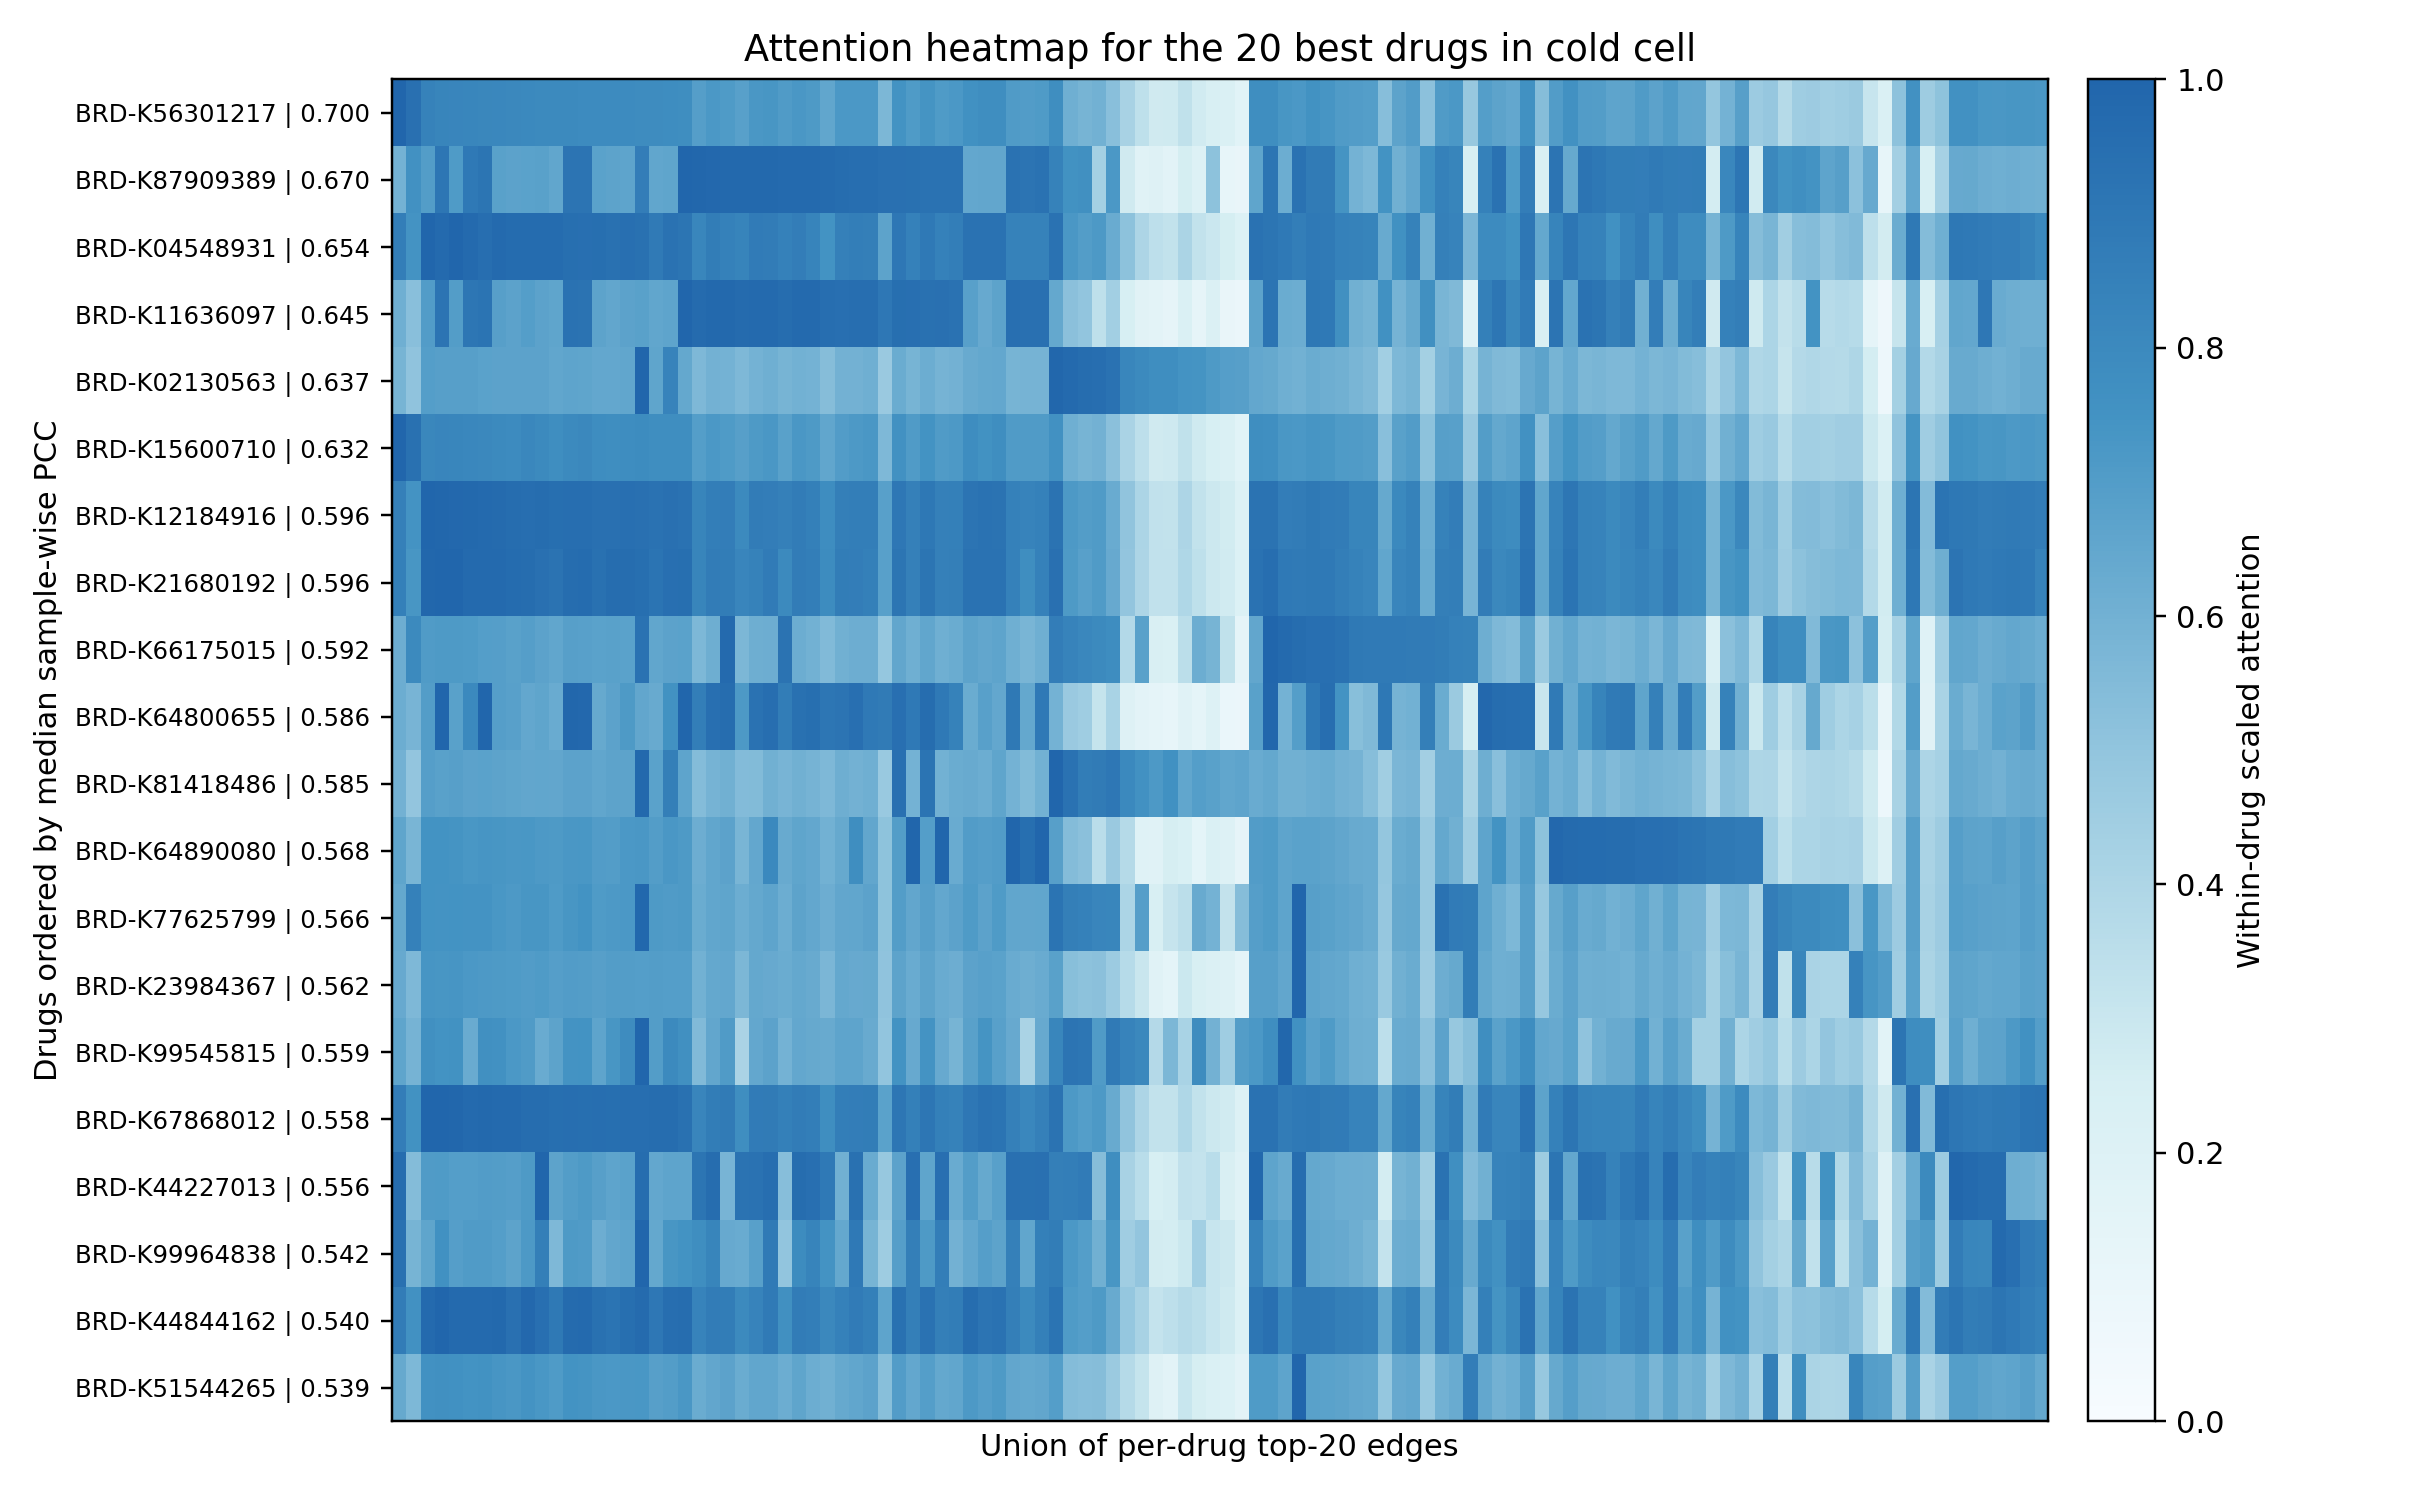
\includegraphics[width=\linewidth]{figures/attention_best_drugs_top20_heatmap_cold_cell.png}
\caption[Best Cold Cell Heatmap]{Attention heatmap for the top 20 best drugs in the cold cell split. For each drug, the heatmap shows the strongest edges between different genes. The values are scaled within each drug. Darker blue regions show where the model puts more attention.}
\label{fig:best_drug_top20_heatmap_cold_cell}
\end{figure}

\noindent Figure~\ref{fig:best_drug_top20_heatmap_cold_cell} shows that several well predicted cold cell drugs still produce clear edge weight patterns even when the cell line is unseen. Some sets of edges reappear across drugs. However, the heatmap alone cannot show whether one specific drug keeps giving high weights to similar edges across warm and cold cell. That question needs a direct comparison of the same drug in both settings.

\noindent Table~\ref{tab:attention_shared_drug_warm_cold_cell} compares the same drug, alvocidib labelled as \texttt{BRD-K87909389}, in warm and cold cell. This drug is reported as a \texttt{CDK inhibitor}. It is an appropriate example because the model performs well on this drug in both settings.

\noindent The table shows a shift in the highly weighted edges. In the warm setting, several top edges involve genes related to cell division, such as \texttt{RB1} and \texttt{E2F2}. In the cold cell setting, more top edges involve genes related to broader stress and damage response, such as \texttt{TP53} and \texttt{NR3C1}. When the cell line is unseen, the model gives more weight to broad response genes than to the more specific genes seen in the warm setting.

\begin{table}[htbp]
\centering
\caption[Shared Drug Edges]{Top high attention edges for one shared drug in warm and cold cell. The same drug, \texttt{BRD-K87909389}, is shown in both settings. The type column indicates whether the prior graph marks the edge as stimulation or inhibition. Attention values come from the last attention layer.}
\label{tab:attention_shared_drug_warm_cold_cell}
\begin{tabular}{lcllcl}
\hline
Warm edge & Type & Attention & Cold cell edge & Type & Attention \\
\hline
\texttt{RB1}$\rightarrow$\texttt{TP53BP2} & stimulation & 0.8077 & \texttt{NR3C1}$\rightarrow$\texttt{TIMELESS} & stimulation & 0.8136 \\
\texttt{HMGA2}$\rightarrow$\texttt{IGF2BP2} & stimulation & 0.8006 & \texttt{TP53}$\rightarrow$\texttt{ASCC3} & stimulation & 0.8044 \\
\texttt{GATA2}$\rightarrow$\texttt{MAPKAPK3} & stimulation & 0.7999 & \texttt{TP53}$\rightarrow$\texttt{CRYZ} & inhibition & 0.7978 \\
\texttt{ELAVL1}$\rightarrow$\texttt{TRIB3} & stimulation & 0.7916 & \texttt{ABL1}$\rightarrow$\texttt{CRKL} & stimulation & 0.7975 \\
\texttt{ELAVL1}$\rightarrow$\texttt{ADAM10} & stimulation & 0.7899 & \texttt{TP53}$\rightarrow$\texttt{P4HA2} & stimulation & 0.7950 \\
\texttt{E2F2}$\rightarrow$\texttt{EED} & stimulation & 0.7892 & \texttt{TP53}$\rightarrow$\texttt{REEP5} & inhibition & 0.7947 \\
\texttt{SMAD3}$\rightarrow$\texttt{BAMBI} & stimulation & 0.7846 & \texttt{PLK1}$\rightarrow$\texttt{SMC1A} & inhibition & 0.7947 \\
\texttt{GATA3}$\rightarrow$\texttt{HAT1} & stimulation & 0.7845 & \texttt{ABL1}$\rightarrow$\texttt{SORBS3} & stimulation & 0.7935 \\
\texttt{PAK1}$\rightarrow$\texttt{PGM1} & stimulation & 0.7836 & \texttt{TP53}$\rightarrow$\texttt{DUSP11} & stimulation & 0.7926 \\
\texttt{GATA3}$\rightarrow$\texttt{BLCAP} & stimulation & 0.7832 & \texttt{TP53}$\rightarrow$\texttt{CCNB2} & inhibition & 0.7919 \\
\texttt{GATA3}$\rightarrow$\texttt{ZW10} & stimulation & 0.7824 & \texttt{TP53}$\rightarrow$\texttt{ITFG1} & stimulation & 0.7857 \\
\texttt{GATA3}$\rightarrow$\texttt{VGLL4} & stimulation & 0.7818 & \texttt{CHEK1}$\rightarrow$\texttt{TLK2} & inhibition & 0.7794 \\
\texttt{HIF1A}$\rightarrow$\texttt{SLC11A2} & stimulation & 0.7817 & \texttt{PLK1}$\rightarrow$\texttt{ZMYM2} & inhibition & 0.7737 \\
\texttt{HIF1A}$\rightarrow$\texttt{ALDOA} & stimulation & 0.7780 & \texttt{HIF1A}$\rightarrow$\texttt{BNIP3} & stimulation & 0.7726 \\
\texttt{HIF1A}$\rightarrow$\texttt{BNIP3} & stimulation & 0.7772 & \texttt{NR3C1}$\rightarrow$\texttt{CEBPD} & stimulation & 0.7639 \\
\texttt{HIF1A}$\rightarrow$\texttt{KDM3A} & stimulation & 0.7770 & \texttt{ELAVL1}$\rightarrow$\texttt{ADAM10} & stimulation & 0.7629 \\
\texttt{TFDP1}$\rightarrow$\texttt{NRIP1} & stimulation & 0.7766 & \texttt{MYC}$\rightarrow$\texttt{PSMG1} & stimulation & 0.7614 \\
\texttt{HIF1A}$\rightarrow$\texttt{S100A4} & stimulation & 0.7699 & \texttt{ELAVL1}$\rightarrow$\texttt{TRIB3} & stimulation & 0.7596 \\
\texttt{MYC}$\rightarrow$\texttt{PAICS} & stimulation & 0.7514 & \texttt{MYC}$\rightarrow$\texttt{UBE2C} & stimulation & 0.7587 \\
\texttt{MYC}$\rightarrow$\texttt{NIT1} & stimulation & 0.7512 & \texttt{HIF1A}$\rightarrow$\texttt{KDM3A} & stimulation & 0.7583 \\
\hline
\end{tabular}
\end{table}

\noindent At the same time, this comparison also shows a limitation. In cold cell, the model does not keep giving high weights to the same specific cell division related edges seen in warm. It still highlights some readable edges, but the result is less specific. This shows that unseen cell lines remain difficult, even when the overall prediction score is good.

\noindent Table~\ref{tab:attention_shared_drug_warm_cold_cell_abt737} gives a second shared drug example, \texttt{BRD-K56301217}. The known targets of this drug are \texttt{BCL2} family proteins.

\noindent The table shows a different result from the alvocidib example. The two highest ranked edges are \texttt{BAX}$\rightarrow$\texttt{VDAC1} and \texttt{BECN1}$\rightarrow$\texttt{PIK3R4}. These two edges stay at the top in both warm and cold cell. Several other edges also overlap between the two settings. The model therefore keeps giving high weights to similar edges even when the cell background changes.

\noindent This consistency is useful when comparing the two settings. In the alvocidib example, the set of high weight edges became broader in cold cell. Here the result is more stable across settings. This shows that the model can keep giving high weights to a similar set of edges across different cell backgrounds for some drugs. 

\begin{table}[htbp]
\centering
\caption[Second Shared Drug Edges]{Top high attention edges for a second shared drug in warm and cold cell. The drug is \texttt{BRD-K56301217}. Its known target genes are \texttt{BCL2}, \texttt{BCL2L1}, and \texttt{BCL2L2}. The type column indicates whether the prior graph marks the edge as stimulation or inhibition. Attention values come from the last attention layer.}
\label{tab:attention_shared_drug_warm_cold_cell_abt737}
\begin{tabular}{lcllcl}
\hline
Warm edge & Type & Attention & Cold cell edge & Type & Attention \\
\hline
\texttt{BECN1}$\rightarrow$\texttt{PIK3R4} & stimulation & 0.7320 & \texttt{BAX}$\rightarrow$\texttt{VDAC1} & stimulation & 0.6833 \\
\texttt{BAX}$\rightarrow$\texttt{VDAC1} & stimulation & 0.7176 & \texttt{BECN1}$\rightarrow$\texttt{PIK3R4} & stimulation & 0.6426 \\
\texttt{RB1}$\rightarrow$\texttt{TP53BP2} & stimulation & 0.5730 & \texttt{SRC}$\rightarrow$\texttt{MAPKAPK5} & stimulation & 0.5716 \\
\texttt{E2F2}$\rightarrow$\texttt{EED} & stimulation & 0.5427 & \texttt{GATA3}$\rightarrow$\texttt{BLCAP} & stimulation & 0.5644 \\
\texttt{GATA2}$\rightarrow$\texttt{MAPKAPK3} & stimulation & 0.5420 & \texttt{E2F2}$\rightarrow$\texttt{EED} & stimulation & 0.5619 \\
\texttt{PCNA}$\rightarrow$\texttt{POLD4} & stimulation & 0.5379 & \texttt{GATA2}$\rightarrow$\texttt{MAPKAPK3} & stimulation & 0.5584 \\
\texttt{HMGA2}$\rightarrow$\texttt{IGF2BP2} & stimulation & 0.5294 & \texttt{GATA3}$\rightarrow$\texttt{VGLL4} & stimulation & 0.5558 \\
\texttt{HIF1A}$\rightarrow$\texttt{KDM3A} & stimulation & 0.5283 & \texttt{SRC}$\rightarrow$\texttt{CLTC} & stimulation & 0.5547 \\
\texttt{GATA3}$\rightarrow$\texttt{ZW10} & stimulation & 0.5272 & \texttt{EGR1}$\rightarrow$\texttt{EAPP} & stimulation & 0.5513 \\
\texttt{HIF1A}$\rightarrow$\texttt{BNIP3} & stimulation & 0.5270 & \texttt{CEBPA}$\rightarrow$\texttt{HSD17B11} & stimulation & 0.5474 \\
\texttt{CEBPA}$\rightarrow$\texttt{HSD17B11} & stimulation & 0.5248 & \texttt{MYLK}$\rightarrow$\texttt{MYL9} & stimulation & 0.5468 \\
\texttt{NFE2L2}$\rightarrow$\texttt{TXNRD1} & stimulation & 0.5248 & \texttt{SRC}$\rightarrow$\texttt{DNM1} & stimulation & 0.5460 \\
\texttt{PHKG2}$\rightarrow$\texttt{PYGL} & stimulation & 0.5238 & \texttt{GATA3}$\rightarrow$\texttt{ZW10} & stimulation & 0.5433 \\
\texttt{CFLAR}$\rightarrow$\texttt{ATG3} & inhibition & 0.5236 & \texttt{GATA3}$\rightarrow$\texttt{HAT1} & stimulation & 0.5410 \\
\texttt{GATA3}$\rightarrow$\texttt{HAT1} & stimulation & 0.5207 & \texttt{CXCR4}$\rightarrow$\texttt{GNAI2} & stimulation & 0.5409 \\
\texttt{SRC}$\rightarrow$\texttt{MAPKAPK5} & stimulation & 0.5186 & \texttt{KIF5C}$\rightarrow$\texttt{TRAK2} & stimulation & 0.5406 \\
\texttt{GATA3}$\rightarrow$\texttt{VGLL4} & stimulation & 0.5186 & \texttt{SRC}$\rightarrow$\texttt{MPZL1} & stimulation & 0.5404 \\
\texttt{NR3C1}$\rightarrow$\texttt{TIMELESS} & stimulation & 0.5181 & \texttt{STAT3}$\rightarrow$\texttt{CSRP1} & stimulation & 0.5357 \\
\texttt{CSNK2A2}$\rightarrow$\texttt{NOL3} & stimulation & 0.5180 & \texttt{STXBP1}$\rightarrow$\texttt{STX1A} & stimulation & 0.5345 \\
\texttt{EGR1}$\rightarrow$\texttt{DUSP4} & stimulation & 0.5175 & \texttt{NFE2L2}$\rightarrow$\texttt{TXNRD1} & stimulation & 0.5316 \\
\hline
\end{tabular}
\end{table}
\noindent Overall, these case studies show that attention can be helpful. When the prediction is strong, the highly weighted edges are often easier to connect to known drug targets or to a later response that looks reasonable. When the prediction is weak, large edge weights can still appear, but they are harder to summarize in a meaningful way. The warm and cold cell comparisons also show two possible results. For some drugs, the model shifts toward broader response genes in unseen cells. For other drugs, it keeps giving high weights to a more similar set of edges. Attention should therefore be interpreted together with prediction quality and prior biological knowledge.
